\documentclass[11pt,a4paper,twoside]{book}\usepackage[]{graphicx}\usepackage[]{xcolor}
% maxwidth is the original width if it is less than linewidth
% otherwise use linewidth (to make sure the graphics do not exceed the margin)
\makeatletter
\def\maxwidth{ %
  \ifdim\Gin@nat@width>\linewidth
    \linewidth
  \else
    \Gin@nat@width
  \fi
}
\makeatother

\definecolor{fgcolor}{rgb}{0.345, 0.345, 0.345}
\newcommand{\hlnum}[1]{\textcolor[rgb]{0.686,0.059,0.569}{#1}}%
\newcommand{\hlsng}[1]{\textcolor[rgb]{0.192,0.494,0.8}{#1}}%
\newcommand{\hlcom}[1]{\textcolor[rgb]{0.678,0.584,0.686}{\textit{#1}}}%
\newcommand{\hlopt}[1]{\textcolor[rgb]{0,0,0}{#1}}%
\newcommand{\hldef}[1]{\textcolor[rgb]{0.345,0.345,0.345}{#1}}%
\newcommand{\hlkwa}[1]{\textcolor[rgb]{0.161,0.373,0.58}{\textbf{#1}}}%
\newcommand{\hlkwb}[1]{\textcolor[rgb]{0.69,0.353,0.396}{#1}}%
\newcommand{\hlkwc}[1]{\textcolor[rgb]{0.333,0.667,0.333}{#1}}%
\newcommand{\hlkwd}[1]{\textcolor[rgb]{0.737,0.353,0.396}{\textbf{#1}}}%
\let\hlipl\hlkwb

\usepackage{framed}
\makeatletter
\newenvironment{kframe}{%
 \def\at@end@of@kframe{}%
 \ifinner\ifhmode%
  \def\at@end@of@kframe{\end{minipage}}%
  \begin{minipage}{\columnwidth}%
 \fi\fi%
 \def\FrameCommand##1{\hskip\@totalleftmargin \hskip-\fboxsep
 \colorbox{shadecolor}{##1}\hskip-\fboxsep
     % There is no \\@totalrightmargin, so:
     \hskip-\linewidth \hskip-\@totalleftmargin \hskip\columnwidth}%
 \MakeFramed {\advance\hsize-\width
   \@totalleftmargin\z@ \linewidth\hsize
   \@setminipage}}%
 {\par\unskip\endMakeFramed%
 \at@end@of@kframe}
\makeatother

\definecolor{shadecolor}{rgb}{.97, .97, .97}
\definecolor{messagecolor}{rgb}{0, 0, 0}
\definecolor{warningcolor}{rgb}{1, 0, 1}
\definecolor{errorcolor}{rgb}{1, 0, 0}
\newenvironment{knitrout}{}{} % an empty environment to be redefined in TeX

\usepackage{alltt}
% We load package by package and set package relevant parameters.
% Topics are summarized later
%%%%%%%%%%%%%%%%%%%%%%%%%%%%%%%%%%%%%%%%%%%%%%%%%%%%%%%%%%%%%%%%%%%%%%%%
% helping packages
\PassOptionsToPackage{dvipsnames}{xcolor}
\usepackage{ifthen}
\usepackage{calc}
\usepackage{geometry}

\usepackage[T1]{fontenc}       % provides fonts having  accented characters 
\usepackage[utf8]{inputenc}  % allows the user to input accented characters directly from the keyboard

%%%%%%%%%%%%%%%%%%%%%%%%%%%%%%%%%%%%%%%%%%%%%%%%%%%%%%%%%%%%%%%%%%%%%%%%

\renewcommand{\baselinestretch}{1.2}
\setlength{\parskip}{0.55\baselineskip}
\setlength{\parindent}{0pt}
\renewcommand{\textfraction}{0}%0.2     % placement of figures
\renewcommand{\topfraction}{1}%.3
\renewcommand{\bottomfraction}{1}%.3
\renewcommand{\floatpagefraction}{1}%.3
\setcounter{bottomnumber}{3}%1

\textwidth6.3in
\textheight9.7in
\topmargin-45pt
\oddsidemargin-.15in
\evensidemargin.15in
\headsep30pt
\headheight15pt
%\footskip20pt


%%%%%%%%%%%%%%%%%%%%%%%%%%%%%%%%%%%%%%%%%%%%%%%%%%%%%%%%%%%%%%%%%%%%%%%%

\usepackage{xcolor}
\definecolor{fgcolor}{rgb}{0.345, 0.345, 0.345}
\definecolor{shadecolor}{rgb}{.97, .97, .97}
\definecolor{messagecolor}{rgb}{0, 0, 0}
\definecolor{warningcolor}{rgb}{1, 0, 1}
\definecolor{errorcolor}{rgb}{1, 0, 0}
\definecolor{DarkBlue}{rgb}{0,0,0.5451}
\definecolor{DarkGreen}{rgb}{0,0.39216,0}
\definecolor{LightYellow}{rgb}{1,1,.8}
\definecolor{orange}{rgb}{.9,0.3445,0}



%%%%%%%%%%%%%%%%%%%%%%%%%%%%%%%%%%%%%%%%%%%%%%%%%%%%%%%%%%%%%%%%%%%%%%%%
\usepackage{afterpage}
\usepackage{natbib}
\usepackage{upquote}

\usepackage[english]{babel}

%%%%%%%%%%%%%%%%%%%%%%%%%%%%%%%%%%%%%%%%%%%%%%%%%%%%%%%%%%%%%%%%%%%%%%%%%%%%%%%
%% maxwidth is the original width if it is less than linewidth
%% otherwise use linewidth (to make sure the graphics do not exceed the margin)
\makeatletter
\def\maxwidth{ %
  \ifdim\Gin@nat@width>\linewidth
    \linewidth
  \else
    \Gin@nat@width
  \fi
}
\makeatother

%%%%%%%%%%%%%%%%%%%%%%%%%%%%%%%%%%%%%%%%%%%%%%%%%%%%%%%%%%%%%%%%%%%%%%%%%%%%%%%%%%%%%%%%%%%%%%%%%%%%%%%%%%%%
% from fancyvrb
\usepackage{fancyhdr}
\usepackage{fancyvrb}
\DefineVerbatimEnvironment{Rcode}{Verbatim}{xleftmargin=2em,fontshape=sl,formatcom=\color{DarkGreen}}
\fvset{listparameters={\setlength{\topsep}{0pt}}}

%%%%%%%%%%%%%%%%%%%%%%%%%%%%%%%%%%%%%%%%%%%%%%%%%%%%%%%%%%%%%%%%%%%%%%%%%%%%%%%%%%%%%%%%%%%%%%%%%%%%%%%%%%%%%
\usepackage{float}
\usepackage{graphicx}
\usepackage{pdflscape}
\usepackage[margin=2em,labelfont=bf]{caption}


%%%%%%%%%%%%%%%%%%%%%%%%%%%%%%%%%%%%%%%%%%%%%%%%%%%%%%%%%%%%%%%%%%%%%%%%
\usepackage[pdftex,plainpages=false,pdfpagelabels,pagebackref=true,colorlinks=true,pdfpagemode=UseOutlines]{hyperref}


%%%%%%%%%%%%%%%%%%%%%%%%%%%%%%%%%%%%%%%%%%%%%%%%%%%%%%%%%%%%%%%%%%%%%%%%
% now math stuff and other details...
\usepackage{amsmath,amsthm,amssymb}
\usepackage{tikz}
\usetikzlibrary{arrows.meta,positioning,calc,matrix}

\newtheorem{pro}{Property}[chapter]
\theoremstyle{definition}
\newtheorem{des}{Definition}[chapter]
\newtheorem{bsp}{Example}[chapter]
\newtheorem{rem}{Remark}[chapter]

\newcommand*\widebar[1]{%
  \vbox{%
    \hrule height 0.5pt%     % Line above with certain width
    \kern0.5ex%             % Distance between line and content
    \hbox{%
      \kern-0.1em%           % Distance between content and left side of box, negative values for lines shorter than content
      \ifmmode#1\else\ensuremath{#1}\fi%  % The content, typeset in dependence of mode
      \kern-0.1em%      % Distance between content and left side of box, negative values for lines shorter than content
    }% end of hbox
  }% end of vbox
}
\def\ds{\displaystyle}

\newcommand{\rr}[1]{{\ttfamily\slshape\color{DarkGreen} #1}}

\makeatletter


% clever trick to circumvent potential redefines after loading packages:
% \providecommand{\something}{}  % if it does not exist, it creates it.
%      has same syntax as \newcommand
% \renewcommand{\something}{....}
% TUGboat 29(2)


\makeatletter
%umdefinierung exisitierender befehle
\let\oldH\H
\let\oldL\L
\let\oldO\H
\let\oldS\S
\let\olda\a
\let\oldb\b
\let\oldc\c
\let\oldd\d
\let\oldk\k
\let\oldv\v
\let\oldl\l
\let\oldt\t
\let\oldu\u
\let\oldIJ\IJ
\let\oldP\P
\let\P\relax
\let\oldnorm\|

%\DefineVerbatimEnvironment{CodeInput}{Verbatim}{fontshape=sl}
%\DefineVerbatimEnvironment{CodeOutput}{Verbatim}{}

% some classical environments, up-right, with chapter numbering.
\theoremstyle{definition}
\newtheorem{definition}{Definition}[chapter]
\newtheorem{example}{Example}[chapter]
\newtheorem{remark}{Remark}[chapter]
\newtheorem{theorem}{Theorem}[chapter]



\renewcommand{\|}{|\!|}         % closer norm
\newcommand{\T}{{}^{\top}}
\newcommand\code[1]{{\tt#1}}



\newcounter{algo}
\newenvironment{algorithm}{%
  \begin{list}{
      (\arabic{algo})
    }{
      \usecounter{algo}
    }%
}{
  \end{list}
}

% some text abbreviation
\newcommand{\GLS}{\text{GLS}}
\newcommand{\RR}{\text{RR}}
\newcommand{\OR}{\text{OR}}
\newcommand{\WLS}{\text{WLS}}
\newcommand{\MLE}{\text{MLE}}
\newcommand{\OLS}{\text{OLS}}
\newcommand{\MAE}{\text{MAE}}
\newcommand{\MAD}{\text{MAD}}
\newcommand{\RMSE}{\text{RMSE}}

\newcommand{\ii}{\text{\i}}

\newcommand{\Bin}{\cB\mathit{\!i\!n}}
\newcommand{\Beta}{\cB\mathit{\!e\!t\!a}}
\newcommand{\Pois}{\cP\mathit{\!o\!i\!s\!s\!o\!n}}
\newcommand{\Exp}{\cE\mathit{\!x\!p}}


\DeclareMathOperator*{\argmin}{argmin}
\DeclareMathOperator*{\argmax}{argmax}
\DeclareMathOperator{\diag}{diag}
\DeclareMathOperator{\diam}{diam}
\DeclareMathOperator{\card}{card}
\DeclareMathOperator{\cov}{Cov}                   
\DeclareMathOperator{\corr}{Corr}                 
\DeclareMathOperator{\var}{Var}                   
\DeclareMathOperator{\trace}{tr}                  
\DeclareMathOperator{\E}{E}                       
\DeclareMathOperator{\P}{P}                       
\DeclareMathOperator{\pred}{p}
\DeclareMathOperator{\vect}{vec}                  
\DeclareMathOperator{\vech}{vech}                 
\DeclareMathOperator{\rank}{rank}                 
\DeclareMathOperator{\e}{e}                       
%\DeclareMathOperator{\cv}{CV}                     
\DeclareMathOperator{\GCV}{GCV}                     
\DeclareMathOperator{\CV}{CV}                     
\DeclareMathOperator{\BLUP}{BLUP}                 
\DeclareMathOperator{\MSE}{MSE}                   
\DeclareMathOperator{\MS}{MS}                   
\DeclareMathOperator{\df}{df}                   
\DeclareMathOperator{\bias}{bias}                   
\DeclareMathOperator{\eig}{eig}                   
\DeclareMathOperator{\Prec}{Prec}
\DeclareMathOperator{\mode}{mode}
\renewcommand{\SS}{\text{SS}}
\renewcommand{\d}{\mathsf{\,d}}

\def\arctanh{\qopname\relax o{arctanh}}  % as in amsopn
\newcommand{\bigo}{\cO}
\newcommand{\lito}{\text{\scriptsize{$\cO$}}}
\newcommand{\cdfPhi}{\itPhi}
\newcommand{\ml}{_\text{ML}}

\newcommand*{\stack@relbin}[3][]{%
  \mathop{#3}\limits
  \toks@{#1}%
  \edef\reserved@a{\the\toks@}%
  \ifx\reserved@a\@empty\else_{#1}\fi
  \toks@{#2}%
  \edef\reserved@a{\the\toks@}%
  \ifx\reserved@a\@empty\else^{#2}\fi
  \egroup
}%
\renewcommand*{\stackrel}{\mathrel\bgroup\stack@relbin}
\newcommand*{\stackbin}{\mathbin\bgroup\stack@relbin}
\newcommand{\simiid}{\stackrel[]{\text{iid}}{\sim}}

% Kalligraphischer Schriftsatz
\newcommand{\cA}{{\cal{A}}}
\newcommand{\cB}{{\cal{B}}} 
\newcommand{\cC}{{\cal{C}}}
\newcommand{\cD}{{\cal{D}}} 
\newcommand{\cE}{{\cal{E}}}
\newcommand{\cF}{{\cal{F}}}
\newcommand{\cG}{{\cal{G}}}
\newcommand{\cH}{{\cal{H}}}
\newcommand{\cI}{{\cal{I}}}
\newcommand{\cJ}{{\cal{J}}}
\newcommand{\cK}{{\cal{K}}}
\newcommand{\cL}{{\cal{L}}}
\newcommand{\cM}{{\cal{M}}} 
\newcommand{\cN}{{\cal{N}}}
\newcommand{\cO}{{\cal{O}}} 
\newcommand{\cP}{{\cal{P}}}
\newcommand{\cQ}{{\cal{Q}}} 
\newcommand{\cR}{{\cal{R}}} 
\newcommand{\cS}{{\cal{S}}} 
\newcommand{\cT}{{\cal{T}}}
\newcommand{\cU}{{\cal{U}}}
\newcommand{\cV}{{\cal{V}}}
\newcommand{\cW}{{\cal{W}}}
\newcommand{\cX}{{\cal{X}}} 
\newcommand{\cY}{{\cal{Y}}}
\newcommand{\cZ}{{\cal{Z}}} 


\newcommand{\IA}{{\mathbb{A}}}
\newcommand{\IB}{{\mathbb{B}}}
\newcommand{\IC}{{\mathbb{C}}}
\newcommand{\ID}{{\mathbb{D}}}
\newcommand{\IE}{{\mathbb{E}}}
\newcommand{\IF}{{\mathbb{F}}}
\newcommand{\IG}{{\mathbb{G}}}
\newcommand{\IH}{{\mathbb{H}}}
\newcommand{\II}{{\mathbb{I}}}
%\newcommand{\IJ}{{\mathbb{J}}}
\newcommand{\IK}{{\mathbb{K}}}
\newcommand{\IL}{{\mathbb{L}}}
\newcommand{\IM}{{\mathbb{M}}}
\newcommand{\IN}{{\mathbb{N}}}
\newcommand{\IO}{{\mathbb{O}}}
\newcommand{\IP}{{\mathbb{P}}}
\newcommand{\IQ}{{\mathbb{Q}}}
\newcommand{\IR}{{\mathbb{R}}}
\newcommand{\IS}{{\mathbb{S}}}
\newcommand{\IT}{{\mathbb{T}}}
\newcommand{\IU}{{\mathbb{U}}}
\newcommand{\IV}{{\mathbb{V}}}
\newcommand{\IW}{{\mathbb{W}}}
\newcommand{\IX}{{\mathbb{X}}}
\newcommand{\IY}{{\mathbb{Y}}}
\newcommand{\IZ}{{\mathbb{Z}}}


% fette griechische kleinbuchstaben
\newcommand{\balpha}{{\boldsymbol{\alpha}}}
\newcommand{\bbeta}{{\boldsymbol{\beta}}}
\newcommand{\bgamma}{{\boldsymbol{\gamma}}}
\newcommand{\bdelta}{{\boldsymbol{\delta}}}
\newcommand{\blambda}{{\boldsymbol{\lambda}}}
\newcommand{\bepsilon}{{\boldsymbol{\epsilon}}}
\newcommand{\bvarepsilon}{{\boldsymbol{\varepsilon}}}
\newcommand{\bzeta}{{\boldsymbol{\zeta}}}
\newcommand{\bfeta}{{\boldsymbol{\eta}}}  %  <----- exception !
\newcommand{\btheta}{{\boldsymbol{\theta}}{}}
\newcommand{\bvartheta}{{\boldsymbol{\vartheta}}}
\newcommand{\biota}{{\boldsymbol{\iota}}}
\newcommand{\bkappa}{{\boldsymbol{\kappa}}}
\newcommand{\bmu}{{\boldsymbol{\mu}}}
\newcommand{\bnu}{{\boldsymbol{\nu}}}
\newcommand{\bxi}{{\boldsymbol{\xi}}}
\newcommand{\bpi}{{\boldsymbol{\pi}}}
\newcommand{\bvarpi}{{\boldsymbol{\varpi}}}
\newcommand{\brho}{{\boldsymbol{\rho}}}
\newcommand{\bvarrhoi}{{\boldsymbol{\varrho}}}
\newcommand{\bsigma}{{\boldsymbol{\sigma}}}
\newcommand{\bvarsigma}{{\boldsymbol{\varsigma}}}
\newcommand{\btau}{{\boldsymbol{\tau}}}
\newcommand{\bvartau}{{\boldsymbol{\vartau}}}
\newcommand{\bupsilon}{{\boldsymbol{\upsilon}}}
\newcommand{\bphi}{{\boldsymbol{\phi}}}
\newcommand{\bvarphi}{{\boldsymbol{\varphi}}}
\newcommand{\bchi}{{\boldsymbol{\chi}}}
\newcommand{\bpsi}{{\boldsymbol{\psi}}}
\newcommand{\bomega}{{\boldsymbol{\omega}}}


% fette griechische grossbuchstaben
\newcommand{\bGamma}{{\boldsymbol{\Gamma}}}
\newcommand{\bDelta}{{\boldsymbol{\Delta}}}
\newcommand{\bTheta}{{\boldsymbol{\Theta}}}
\newcommand{\bLambda}{{\boldsymbol{\Lambda}}{}}
\newcommand{\bXi}{{\boldsymbol{\Xi}}}
\newcommand{\bPi}{{\boldsymbol{\Pi}}}
\newcommand{\bSigma}{{\boldsymbol{\Sigma}}{}}
\newcommand{\bUpsilon}{{\boldsymbol{\Upsilon}}{}}
\newcommand{\bPhi}{{\boldsymbol{\Phi}}}
\newcommand{\bPsi}{{\boldsymbol{\Psi}}}
\newcommand{\bOmega}{{\boldsymbol{\Omega}}}

% italics griechische grossbuchstaben
\newcommand{\itGamma}{{\mathit{\Gamma}}}
\newcommand{\itDelta}{{\mathit{\Delta}}}
\newcommand{\itTheta}{{\mathit{\Theta}}}
\newcommand{\itLambda}{{\mathit{\Lambda}}}
\newcommand{\itXi}{{\mathit{\Xi}}}
\newcommand{\itPi}{{\mathit{\Pi}}}
\newcommand{\itSigma}{{\mathit{\Sigma}}}
\newcommand{\itUpsilon}{{\mathit{\Upsilon}}}
\newcommand{\itPhi}{{\mathit{\Phi}}}
\newcommand{\itPsi}{{\mathit{\Psi}}}
\newcommand{\itOmega}{{\mathit{\Omega}}}



\newcommand{\A}{{\mathbf{A}}}
\newcommand{\B}{{\mathbf{B}}}
\newcommand{\C}{{\mathbf{C}}}
\newcommand{\D}{{\mathbf{D}}}
\newcommand{\bfE}{{\mathbf{E}}}    % \E: expectation
\newcommand{\F}{{\mathbf{F}}}
\newcommand{\G}{{\mathbf{G}}}
\renewcommand{\H}{{\mathbf{H}}}
\newcommand{\I}{{\mathbf{I}}}
\newcommand{\J}{{\mathbf{J}}}
\newcommand{\K}{{\mathbf{K}}}
\renewcommand{\L}{{\mathbf{L}}}
\newcommand{\bfM}{{\mathbf{M}}}
\newcommand{\N}{{\mathbf{N}}}
\renewcommand{\O}{{\mathbf{O}}}
\newcommand{\bfP}{{\mathbf{P}}}  % \P : probability
\newcommand{\Q}{{\mathbf{Q}}}
\newcommand{\bfR}{{\mathbf{R}}}
\renewcommand{\S}{{\mathbf{S}}}
\newcommand{\bfT}{{\mathbf{T}}} % \T transpose
\newcommand{\U}{{\mathbf{U}}}
\newcommand{\V}{{\mathbf{V}}}
\newcommand{\W}{{\mathbf{W}}}
\newcommand{\X}{{\mathbf{X}}}
\newcommand{\Y}{{\mathbf{Y}}}
\newcommand{\Z}{{\mathbf{Z}}}


\newcommand{\0}{{\mathbf{0}}}
\newcommand{\1}{{\mathbf{1}}}
\newcommand{\2}{{\mathbf{2}}}
\newcommand{\3}{{\mathbf{3}}}
\newcommand{\4}{{\mathbf{4}}}
\newcommand{\5}{{\mathbf{5}}}
\newcommand{\6}{{\mathbf{6}}}
\newcommand{\7}{{\mathbf{7}}}
\newcommand{\8}{{\mathbf{8}}}
\newcommand{\9}{{\mathbf{9}}}

\renewcommand{\a}{{\textbf{\textit{a}}}}
\renewcommand{\b}{{\textbf{\textit{b}}}}
\renewcommand{\c}{{\textbf{\textit{c}}}}
\newcommand{\bfd}{{\textbf{\textit{d}}}}  % \d  'dx'
\newcommand{\bfe}{{\textbf{\textit{e}}}}  % \e  l'exponentiel
\newcommand{\f}{{\textbf{\textit{f}}}}
\newcommand{\g}{{\textbf{\textit{g}}}}
\newcommand{\h}{{\textbf{\textit{h}}}}
\newcommand{\bfi}{{\textbf{\textit{i}}}}%\i  complex i, sans 'dot'
\newcommand{\bfj}{{\textbf{\textit{j}}}}
\renewcommand{\l}{{\textbf{\textit{l}}}}
\renewcommand{\k}{{\textbf{\textit{k}}}}
\newcommand{\m}{{\textbf{\textit{m}}}}
\newcommand{\bfn}{{\textbf{\textit{n}}}}
\newcommand{\bfo}{{\textbf{\textit{o}}}}
\newcommand{\p}{{\textbf{\textit{p}}}}
\newcommand{\q}{{\textbf{\textit{q}}}}
\renewcommand{\r}{{\textbf{\textit{r}}}}
\newcommand{\s}{{\textbf{\textit{s}}}}
\renewcommand{\t}{{\textbf{\textit{t}}}}
\newcommand{\bfu}{{\textbf{\textit{u}}}} %\u used in references
\renewcommand{\v}{{\textbf{\textit{v}}}}
\newcommand{\w}{{\textbf{\textit{w}}}}
\newcommand{\x}{{\textbf{\textit{x}}}}
\newcommand{\y}{{\textbf{\textit{y}}}}
\newcommand{\z}{{\textbf{\textit{z}}}}




\ifcsname hlkwd\endcsname%    ... command '#1' exists ...%
  % in this case, it seems that knitr.sty is loaded.
\else%  ... command '#1' does not exist ...%

\def\maxwidth{ %
  \ifdim\Gin@nat@width>\linewidth
    \linewidth
  \else
    \Gin@nat@width
  \fi
}

\definecolor{fgcolor}{rgb}{0.345, 0.345, 0.345}
\newcommand{\hlnum}[1]{\textcolor[rgb]{0.686,0.059,0.569}{#1}}%
\newcommand{\hlstr}[1]{\textcolor[rgb]{0.192,0.494,0.8}{#1}}%
\newcommand{\hlcom}[1]{\textcolor[rgb]{0.678,0.584,0.686}{\textit{#1}}}%
\newcommand{\hlopt}[1]{\textcolor[rgb]{0,0,0}{#1}}%
\newcommand{\hlstd}[1]{\textcolor[rgb]{0.345,0.345,0.345}{#1}}%
\newcommand{\hlkwa}[1]{\textcolor[rgb]{0.161,0.373,0.58}{\textbf{#1}}}%
\newcommand{\hlkwb}[1]{\textcolor[rgb]{0.69,0.353,0.396}{#1}}%
\newcommand{\hlkwc}[1]{\textcolor[rgb]{0.333,0.667,0.333}{#1}}%
\newcommand{\hlkwd}[1]{\textcolor[rgb]{0.737,0.353,0.396}{\textbf{#1}}}%
% In knitr version 1.47, \hlstr and \hlstr have been
% renamed to \hlsng and \hldef respectively. Here, we define all four.
% https://github.com/yihui/knitr/releases/tag/v1.47
\newcommand{\hlsng}[1]{\textcolor[rgb]{0.192,0.494,0.8}{#1}}%
\newcommand{\hldef}[1]{\textcolor[rgb]{0.345,0.345,0.345}{#1}}%


\usepackage{framed}
\newenvironment{kframe}{%
 \def\at@end@of@kframe{}%
 \ifinner\ifhmode%
  \def\at@end@of@kframe{\end{minipage}}%
  \begin{minipage}{\columnwidth}%
 \fi\fi%
 \def\FrameCommand##1{\hskip\@totalleftmargin \hskip-\fboxsep
 \colorbox{shadecolor}{##1}\hskip-\fboxsep
     % There is no \\@totalrightmargin, so:
     \hskip-\linewidth \hskip-\@totalleftmargin \hskip\columnwidth}%
 \MakeFramed {\advance\hsize-\width
   \@totalleftmargin\z@ \linewidth\hsize
   \@setminipage}}%
 {\par\unskip\endMakeFramed%
 \at@end@of@kframe}
% The above is taken verbatim from knitr.sty. Below a modified one, being less
% space resource demanding. Note the \fboxsep -> 0\fboxsep
\renewenvironment{kframe}{%
 \def\at@end@of@kframe{}%
 \ifinner\ifhmode%
  \def\at@end@of@kframe{\end{minipage}}%
  \begin{minipage}{\columnwidth}%
 \fi\fi%
 \def\FrameCommand##1{\hskip\@totalleftmargin \hskip-0\fboxsep
 \colorbox{shadecolor}{##1}\hskip-0\fboxsep
     % There is no \\@totalrightmargin, so:
     \hskip-\linewidth \hskip-\@totalleftmargin \hskip\columnwidth}%
 \MakeFramed {\advance\hsize-\width
   \@totalleftmargin\z@ \linewidth\hsize
   \@setminipage}}%
 {\par\unskip\endMakeFramed%
 \at@end@of@kframe}


\definecolor{shadecolor}{rgb}{.97, .97, .97}
\definecolor{messagecolor}{rgb}{0, 0, 0}
\definecolor{warningcolor}{rgb}{1, 0, 1}
\definecolor{errorcolor}{rgb}{1, 0, 0}
%\newenvironment{knitrout}{}{} % an empty environment to be redefined in TeX
\newenvironment{knitrout}{\setlength{\topsep}{0mm}\setlength{\fboxsep}{4mm}}{} 

\usepackage{alltt}
\IfFileExists{upquote.sty}{\usepackage{upquote}}{}

  \fi%

\makeatother
   % packages, layout and standard macros
\IfFileExists{upquote.sty}{\usepackage{upquote}}{}
\begin{document}
% Title page template for Master Thesis in Biostatistics
\begin{titlepage}
\newgeometry{
  a4paper,
  top=36mm,
  left=25mm,
  right=25mm,
  bottom=24mm,
  headsep=26mm,
  footskip=15mm
}
\thispagestyle{empty}
\renewcommand\familydefault{\sfdefault}
\renewcommand{\baselinestretch}{1.5}\normalfont
\begin{center}
  \setlength{\parindent}{0cm}
  {\bfseries\Large
  Multivariate Density Estimation\\
  Comparing Transformation Forests, Triangular Transport Maps, and Copulas\par}

  \vspace{2mm}
  \hrulefill

  \vspace*{4cm}

  {\large Master Thesis in Biostatistics (STA495)\par}

  \vspace*{12mm}
  by

  \vspace*{12mm}
  Léon Kia Faro \\
  {\small 13-795-026\par}

  \vspace*{4cm}
  supervised by

  \vspace*{12mm}
  Prof. Dr. Torsten Hothorn

  \vfill
  Zurich, September 2025 
\end{center}
\renewcommand\familydefault{\rmdefault}
\renewcommand{\baselinestretch}{1.0}\rmfamily
\setcounter{page}{0}
\end{titlepage}
\restoregeometry
\cleardoublepage





\graphicspath{{./figure/}}
\DeclareGraphicsExtensions{.pdf,.png}
\frontmatter
\pagenumbering{roman}
\setcounter{tocdepth}{1}

\chapter*{Abstract}

This thesis evaluates three approaches to multivariate density estimation for tabular data within a single, consistent pipeline: separable triangular transport maps (TTM-Sep), Transformation Random Forests (TRTF), and copulas. All methods use standardized inputs and a common evaluation protocol so that likelihoods and diagnostics are directly comparable; compute summaries are reported for TRTF (Table~3.7). In the configuration studied, TRTF and TTM-Sep yield the same triangular-likelihood form, which enables like-for-like evaluation. Separable triangular maps deliver exact likelihoods, O(K) evaluation/inversion, and transparent conditionals, but restrict context-dependent shape.


On Half-Moon ($n=250$), mean joint negative log-likelihoods (NLL; lower is better) were $1.71$ (TRTF), $1.93$ (TTM-Sep), and $1.54$ (copula). On a four-dimensional autoregressive generator they were $4.53$, $5.66$, and $5.45$, respectively; permutation averages confirm order sensitivity for triangular maps. On MiniBooNE ($K=43$; mean test log-likelihood per sample), TRTF reached $-30.01$ under the standard preprocessing and training budget used here; published flow models report values around $-12$ to $-16$ under their settings. These numbers are not strictly comparable but indicate the relative accuracy of this configuration.

Overall, TRTF tends to lead within the separable family at low dimension, while higher-dimensional datasets expose the limits of separable structure. We report robustness checks (ordering), calibration diagnostics, and the numerical safeguards used, and we outline directions toward richer parameterizations within the same evaluation frame.

\tableofcontents
\setkeys{Gin}{width=.8\textwidth}

\cleardoublepage
\mainmatter


%%%%%%%%%%%%%%%%%%%%%%%%%%%%%%%%%%%%%%%%%%%%%%%%%%%%%%%%%%%%%%%%%%%%%%


% LaTeX file for Chapter 01


\chapter{Introduction}\label{ch:intro}

Multivariate density estimation is a cornerstone of modern statistics and machine learning. It supplies the machinery for likelihood-based inference, simulation of generative mechanisms, and uncertainty quantification in tabular domains. Practitioners, however, routinely face a delicate trade-off between three goals: expressive power, computational feasibility, and interpretability. Three complementary families of estimators have emerged around this dilemma:
\begin{enumerate}
  \item \textbf{Normalizing flows} build expressive change-of-variables maps and have become central in deep generative modeling \citep{rezende2015variational,papamakarios2017masked,dinh2017real,durkan2019neural,kingma2018glow,papamakarios2021normalizing}.
  \item \textbf{Transformation models and forests} model conditional distributions through parametric transformation structures coupled with ensemble methods \citep{hothorn2017transformation,hothorn2018conditional,hothorn2021transformation}.
  \item \textbf{Copulas} separate marginals from dependence, yielding interpretable multivariate association models \citep{sklar1959fonctions,nelsen2006introduction,joe2014dependence,nagler2017kdecopula}.
\end{enumerate}

This thesis situates all three families inside a common \textbf{transport framework} that makes them directly comparable \citep{rosenblatt1952remarks,knothe1957contributions,bogachev2005triangular,ramgraber2025friendly}. The framework operates in standardized coordinates $u$ computed solely from training-split statistics to avoid leakage and keep objectives aligned across models. Within this evaluation framework each estimator couples $u$ to a reference distribution---Gaussian for triangular maps and TRTF, $\mathrm{Unif}([0,1]^K)$ for copulas---and recovers densities via exact change of variables. Section~\ref{sec:ch1-frame} previews the core pieces and Chapter~\ref{ch:background} develops the mathematics in detail.

Separable triangular transport maps play a central role throughout the thesis. Their lower-triangular Jacobian delivers a log-determinant in $\mathcal{O}(K)$ operations, back-substitution yields an explicit inverse for sampling, and the triangular structure produces exact conditional densities in a fixed order. Fully triangular maps can require $\mathcal{O}(K^2)$ work per evaluation, whereas separable variants reduce both forward and inverse passes to $\mathcal{O}(K)$, making them attractive for systematic comparison while preserving interpretable marginals and dependence mechanisms.

\medskip
\noindent\textit{Notation.} We write $\varphi$ and $\Phi$ for the density and cumulative distribution function of a univariate standard normal random variable, and $\eta$ for the $K$-variate standard normal density. All models are evaluated in standardized coordinates $u$ and reported on the original scale $x$ through a diagonal affine correction so that log densities remain comparable.

\section{Thesis and Problem Statement}\label{sec:ch1-problem}

Let $u = D^{-1}(x - \mu)$ with $D = \mathrm{diag}(\sigma_1,\ldots,\sigma_K)$ determined from the training split. If $T: \mathbb{R}^K \to \mathbb{R}^K$ is lower triangular, $z = T(u)$, and $\eta$ denotes the chosen reference density, then the change-of-variables formula gives
\begin{equation}
  \log p_X(x) = \log \eta\big(T(u)\big) + \sum_{k=1}^{K} \log \frac{\partial T_k}{\partial u_k}(u_{1:k}) - \sum_{k=1}^{K} \log \sigma_k,
  \label{eq:ch1-change-of-variables}
\end{equation}
so reporting on the $x$-scale differs from reporting on the $u$-scale by the constant $-\sum_k \log \sigma_k$ per data point. We standardize elementwise via $u_k = \frac{x_k-\mu_k}{\sigma_k}$ for $k=1,\dots,K$, equivalently $u = \operatorname{diag}(\sigma)^{-1}(x-\mu)$. We write $u_{1:k} = (u_1,\dots,u_k)$ for the prefix subvector.

The Rosenblatt and Knothe rearrangements guarantee the existence of such triangular transports for any coordinate ordering \citep{rosenblatt1952remarks,knothe1957contributions}.

The copula baselines considered here are nonparametric kernel copulas \citep{nagler2017kdecopula}. We fit smooth univariate marginals with \texttt{kde1d}, form pseudo-observations using mid-rank empirical CDFs during training to avoid double smoothing, and evaluate joint densities through
\[
  p_X(x) = c\big(F_1(x_1),\ldots,F_K(x_K)\big)\, \prod_{k=1}^{K} f_k(x_k),
\]
where $c$ is the copula density and $F_k = \int f_k$ the smoothed marginal CDFs. No Gaussian copula enters the study, and the emphasis remains on flexible, interpretable diagnostics in low dimensions.

Separable triangular maps decompose each coordinate into a context-dependent shift plus a one-dimensional monotone transform. TRTF occupies an intermediate position: under strictly increasing conditional CDFs and the standard forest aggregation after monotone smoothing it reproduces the same separable triangular likelihood via the probability integral transform. The shared protocol described above keeps preprocessing, likelihood evaluation, calibration diagnostics, and compute measurements aligned across all estimators.

\section{The Transport Frame on One Page}\label{sec:ch1-frame}

The key ingredients of the transport framework are:
\begin{itemize}
  \item \textbf{Standardization.} Coordinates $u = D^{-1}(x-\mu)$ use training-split statistics only, and all logs use the natural logarithm.
  \item \textbf{Change of variables.} Densities follow from $z = T(u)$ through Equation~\eqref{eq:ch1-change-of-variables}.
  \item \textbf{Triangular log determinant.} Lower-triangular Jacobians imply $\log \det J_T(u) = \sum_k \log \partial_{u_k} T_k(u_{1:k})$, giving $\mathcal{O}(K)$ cost.
  \item \textbf{Affine correction.} Reporting on $x$ applies the constant correction $-\sum_k \log \sigma_k$ per data point.
  \item \textbf{Computational profile.} Fully triangular maps can incur $\mathcal{O}(K^2)$ evaluation and inversion, whereas separable maps reduce both passes to $\mathcal{O}(K)$ while keeping the log determinant linear in $K$.
\end{itemize}

Separable triangular transports implement each coordinate as the sum of a context shift and a monotone one-dimensional basis, maintaining determinant stability and consistent conditional behaviour. TRTF achieves the same likelihood under the conditions noted above, while nonparametric copulas operate on the unit hypercube with explicit marginals. Standardization $u = T_{\mathrm{std}}(x)$ feeds either the triangular transport branch (TTM variants, TRTF) or the copula branch, and both return log densities, conditional diagnostics, samples, and calibration metrics.

\section{Contributions and Research Questions}\label{sec:ch1-contributions}

The thesis contributes along three axes that move from theoretical unification to empirical benchmarking and practical interpretation:
\begin{enumerate}
  \item \textbf{Unified likelihood framework.} We formalise a shared transport perspective that places separable triangular maps, TRTF, and nonparametric copulas inside one mathematical scheme. The equivalence between TRTF and separable triangular transports holds under explicit regularity assumptions---strictly monotone conditional CDFs and the forest aggregation after smoothing.

    \begin{quote}
    \textbf{Proposition (informal).} Under axis-parallel partitions, strictly monotone conditional CDFs, and the forest aggregation after smoothing, the TRTF likelihood coincides with that of a separable triangular transport in standardized coordinates.
    \end{quote}

  \item \textbf{Benchmarking under a common protocol.} We design a standardized evaluation pipeline covering synthetic generators and real tabular benchmarks. TTM-Sep, its marginal variant, and TRTF are evaluated systematically, and nonparametric kernel copulas act as diagnostic comparators when $K \le 3$. The pipeline produces two categories of evidence: (i) average test log likelihoods and (ii) conditional diagnostics based on probability integral transforms. Together they quantify the trade-offs among accuracy and calibration.

  \item \textbf{Operational insights.} The theoretical and empirical findings yield guidance for practitioners. We analyse sensitivity to ordering, the practical limits of separability, and when nonparametric copulas remain informative as diagnostic references. Chapter~\ref{ch:conclusion} synthesizes these insights and outlines extensions toward richer parameterisations.
\end{enumerate}

Two research questions organise the empirical study:
\begin{itemize}
  \item \textbf{Synthetic data.} We investigate how TRTF, TTM-Sep, and nonparametric copulas compare on controlled generators. Evidence comprises likelihood comparisons and conditional calibration metrics.
  \item \textbf{Benchmark datasets.} We assess how close TRTF results come to published normalizing flow baselines under identical preprocessing. Side-by-side likelihood comparisons, interpreted through the constraints of separability, answer this question.
\end{itemize}

\begin{table}[t]
  \centering
  \caption{Model abbreviations used throughout the thesis.}
  \label{tab:model-abbrev}
  \begin{tabular}{ll}
    \hline
    Label & Meaning \\
    \hline
    TTM-Marg  & Marginal triangular transport (per-dimension, no context) \\
    TTM-Sep   & Separable triangular transport (context shift $+$ monotone 1D transform) \\
    TRTF      & Transformation Random Forests (axis-parallel splits) \\
    True-Marg & Oracle marginal density \\
    True-Joint& Oracle conditional joint density \\
    Copula    & Nonparametric kernel copula baseline \\
    \hline
  \end{tabular}
\end{table}

Addressing these questions bridges rigorous transport-based theory with empirical validation, clarifying when simple triangular models suffice and when more expressive families become necessary.

%%%%%%%%%%%%%%%%%%%%%%%%%%%%%%%%%%%%%%%%%%%%%%%%%%%%%%%%%%%%%%%%%%%%%%



% LaTeX file for Chapter 02


\chapter{Methodological Background}\label{ch:background}

\section{Transport Framework and Notation}\label{sec:transport-frame}

This section establishes the coordinate system, notation, and algebraic identities used throughout the thesis. The schematic in Appendix~\ref{ch:appendix} remains valid. Here we focus only on the formulas that are needed later. We set up the standardized pullback likelihood, the triangularity assumption, and the Jacobian factorization.

We write $u_{1:k}=(u_1,\ldots,u_k)$ and use $\partial_{u_k}$ for partial derivatives with respect to $u_k$.

We observe data on the original scale $x \in \mathbb{R}^K$. Training-split statistics define a fixed standardization map
\begin{equation}
  u \;=\; T_{\mathrm{std}}(x) \;=\; (x-\mu)\oslash\sigma,\qquad \sigma_k>0,
  \label{eq:transport-standardise}
\end{equation}
where $\mu$ and $\sigma$ are the empirical mean and standard deviation estimated on the training split, and $\oslash$ denotes elementwise division. Each feature is shifted and rescaled once using training data only. All derivatives and Jacobians are then taken in $u$-space, which avoids leakage and keeps results comparable across estimators.

We model $\pi_U$ as the pullback of a simple reference $\eta$ through a triangular map $S:u\mapsto z$. The reference is the $K$-variate standard normal $\eta(z)$. Applying the change-of-variables formula gives
\begin{equation}
  \pi_U(u) \;=\; \eta\!\left(S(u)\right)\,\left|\det\nabla_u S(u)\right|.
  \label{eq:transport-pullback}
\end{equation}

To report log densities on the original scale, we apply only the diagonal affine correction implied by standardization:
\begin{equation}
  \log \pi_X(x) \;=\; \log \pi_U\!\left(T_{\mathrm{std}}(x)\right) - \sum_{k=1}^{K}\log\sigma_k.
  \label{eq:transport-affine}
\end{equation}

The transport is assumed to be lower triangular and strictly increasing in each coordinate,
\begin{equation}
  S(u) \;=\; \big(S_1(u_1), S_2(u_{1:2}), \ldots, S_K(u_{1:K})\big), 
  \qquad \partial_{u_k}S_k(u_{1:k})>0,
  \label{eq:transport-triangular}
\end{equation}
so the Jacobian $\nabla_u S(u)$ is lower triangular. Its determinant factorizes as
\begin{equation}
  \log \big|\det \nabla_u S(u)\big| \;=\; \sum_{k=1}^{K}\log \partial_{u_k}S_k(u_{1:k}).
  \label{eq:transport-det}
\end{equation}

This factorization makes the \emph{log-determinant} cost $\mathcal{O}(K)$ once the diagonal terms are available. Evaluating all $S_k(u_{1:k})$ can be $\mathcal{O}(K^2)$ for a general triangular map, but reduces to $\mathcal{O}(K)$ in the separable parameterization of Section~\ref{sec:transport-separable}.

Strict monotonicity on each coordinate ($\partial_{u_k} S_k>0$) together with triangularity implies that $S$ is a bijection with a triangular inverse, computable by back-substitution.

\begin{table}[t]
  \centering
  \caption{Notation for the transport framework used in Chapters~\ref{ch:background} and~\ref{ch:dataanalysis}. All derivatives and Jacobians are with respect to $u$. Log densities on $x$ apply the affine correction in Equation~\eqref{eq:transport-affine}.}
  \label{tab:transport-notation}
  \begin{tabular}{@{} l p{0.55\linewidth} l @{}}
    \hline
    Symbol & Meaning & Dimension/Shape \\
    \hline
    $x$ & Original features on the data scale & $\mathbb{R}^K$ \\
    $T_{\mathrm{std}}$ & Standardization map using training $(\mu,\sigma)$ & $\mathbb{R}^K \to \mathbb{R}^K$ \\
    $u = T_{\mathrm{std}}(x)$ & Standardized evaluation coordinates & $\mathbb{R}^K$ \\
    $u_{1:k}$ & Prefix subvector $(u_1,\dots,u_k)$ & $\mathbb{R}^k$ \\
    $z$ & Reference coordinates after transport & $\mathbb{R}^K$ \\
    $S: u \mapsto z$ & Monotone lower-triangular transport map & $\mathbb{R}^K \to \mathbb{R}^K$ \\
    $\nabla_u S(u)$ & Jacobian of $S$ (lower triangular) & $\mathbb{R}^{K \times K}$ \\
    $\eta(z)$ & $K$-variate standard normal density & $\mathbb{R}^K \to \mathbb{R}_{\ge 0}$ \\
    $\varphi(t)$, $\Phi(t)$ & Univariate standard normal density and CDF & $\mathbb{R} \to \mathbb{R}_{\ge 0}$; $\mathbb{R} \to (0,1)$ \\
    $\pi_U$, $\pi_X$ & Densities on $u$- and $x$-space & $\mathbb{R}^K \to \mathbb{R}_{\ge 0}$ \\
    $\mu$, $\sigma$ & Training mean vector and positive scales & $\mathbb{R}^K$ \\
    $K$ & Dimension of the feature vector & $K \in \mathbb{N}$ \\
    \hline
  \end{tabular}
\end{table}


Taken together, the triangular and strictly monotone structure turns joint density evaluation
and sampling into sequential one-dimensional stages, and the standardized coordinates allow us
to report on the $x$-scale with only the diagonal correction from Equation~\eqref{eq:transport-affine}.

\section{Triangular Maps and Transformation Random Forests}\label{sec:transport-separable}

We now move from the general triangular setup to the first concrete parameterization: the separable triangular map. We then show how Transformation Random Forests (TRTF) fit into the same framework. The aim is a shared likelihood that we can train, compare, and diagnose across estimators without changing conventions.

\subsection{Separable triangular component}

A separable component has the form
\begin{equation}
  S_k(u_{1:k}) \;=\; g_k(u_{1:k-1}) + h_k(u_k), \qquad h_k'(u_k) > 0,
  \label{eq:transport-separable}
\end{equation}
where earlier coordinates shift location through $g_k$, while $h_k$ shapes the marginal and ensures monotonicity. To fix identifiability, we enforce a convention such as centering $g_k$ on the training split, $\mathbb E[g_k(U_{1:k-1})]=0$.

With the standard normal reference, the pullback identity becomes
\begin{equation}
  \log \pi_U(u) \;=\; \sum_{k=1}^{K}\Big[\log \varphi\!\big(S_k(u_{1:k})\big) + \log h_k'(u_k)\Big].
  \label{eq:transport-likelihood}
\end{equation}
Up to a constant, the per-sample negative log-likelihood is
\begin{equation}
  \mathcal{L}(u) \;=\; \sum_{k=1}^{K}\Big[\tfrac{1}{2}\,S_k(u_{1:k})^2 - \log h_k'(u_k)\Big].
  \label{eq:transport-loss}
\end{equation}

For a dataset $\{u^{(i)}\}_{i=1}^n$, the empirical objective reads
\[
\mathcal L_n = \frac{1}{n}\sum_{i=1}^n \sum_{k=1}^{K}
\Big[\tfrac{1}{2}\,S_k(u^{(i)}_{1:k})^2 - \log h_k'(u^{(i)}_k)\Big] + \text{const}.
\]

These formulas evaluate in $\mathcal{O}(K)$ time per sample, since the Jacobian term depends only on $u_k$. Sampling inverts $S$ by back-substitution, and log densities on $x$-space apply the affine correction in Equation~\eqref{eq:transport-affine}. The speed comes with a trade-off: separability fixes the conditional shape along $u_k$ once $g_k$ shifts the location, so variance, skewness, and modality no longer adapt to the context $u_{1:k-1}$.

\subsection{Transformation Random Forests in the framework}\label{sec:transport-trtf}

Transformation Random Forests (TRTF) fit conditional CDFs and insert them into the triangular pipeline via the probability integral transform. Let $\widehat F_k(\cdot \mid u_{1:k-1})$ denote the smoothed conditional CDF. Define
\begin{equation}
  S_k(u_{1:k}) \;=\; \Phi^{-1}\!\Big(\widehat F_k(u_k \mid u_{1:k-1})\Big).
  \label{eq:transport-trtf-map}
\end{equation}

If the forest is parameterized additively as
\begin{equation}
  \widehat F_k(u_k \mid u_{1:k-1}) \;=\; \Phi\!\big(h_k(u_k) + g_k(u_{1:k-1})\big),
  \label{eq:transport-trtf-additive}
\end{equation}
then we recover the separable structure,
\begin{equation}
  S_k(u_{1:k}) \;=\; h_k(u_k) + g_k(u_{1:k-1}), \qquad h_k'(u_k) > 0.
  \label{eq:transport-trtf-separable}
\end{equation}


\[
\partial_{u_k}S_k
= \frac{d}{du_k}\Phi^{-1}(\Phi(h_k(u_k)+g_k))
= h_k'(u_k) > 0,
\]
so the Jacobian diagonal is indeed $h_k'(u_k)$ in the additive TRTF case.


In practice, forests may produce $\widehat F_k$ values outside $(0,1)$ by tiny amounts or with imperfect monotonicity. We therefore clip to $(\varepsilon,1-\varepsilon)$ with $\varepsilon=10^{-6}$ and, if needed, apply isotonic post-processing to enforce strict increase. This keeps $S_k=\Phi^{-1}(\widehat F_k)$ well defined.

With this forest aggregation and strictly monotone conditionals, the resulting TRTF map coincides with the separable parameterization, so it delivers the same likelihood and back-substitution sampler.

\section{Copula Baselines}\label{sec:transport-copula}

Standardization remains global (based on the full training split), whereas marginal fits for copulas are per-class. This ensures comparability on the $x$-scale when reporting.



For each class $y$, we proceed as follows:

\begin{itemize}
  \item \textbf{Marginals:} Fit univariate kernel densities (\texttt{kde1d}) to obtain $\widehat f_k(\cdot \mid y)$ and CDFs $\widehat F_k(\cdot \mid y)$.
  \item \textbf{Pseudo-observations:} Transform samples to $(0,1)$ using mid-ranks,
  \begin{equation}
    U_{ik}^{(y)} \;=\; \frac{\operatorname{rank}(X_{ik}^{(y)})}{n_y + 1}.
    \label{eq:copula-midranks}
  \end{equation}
Mid-ranks handle ties. If the data contain many, a tiny jitter is added before ranking.
  \item \textbf{Dependence:} Fit a bivariate kernel copula density $c_y(u_1,u_2)$ using \texttt{kdecopula::kdecop} with local quadratic smoothing, which uses a transformation approach to avoid boundary bias \citep{nagler2017kdecopula}.
\end{itemize}

For prediction at $x=(x_1,x_2)$:
\begin{enumerate}
  \item Evaluate $\widehat f_k(x_k \mid y)$ and $\widehat F_k(x_k \mid y)$.
  \item Evaluate $c_y(\widehat F_1(x_1\mid y), \widehat F_2(x_2\mid y))$.
  \item Combine them through
  \begin{equation}
    \log \widehat \pi_X(x \mid Y=y) 
      \;=\; \log \widehat f_1(x_1 \mid y) + \log \widehat f_2(x_2 \mid y)
      + \log c_y\!\Big(\widehat F_1(x_1 \mid y), \widehat F_2(x_2 \mid y)\Big).
    \label{eq:copula-logdensity}
  \end{equation}
\end{enumerate}
When labels are unknown, we mix across classes using priors $\pi(y)$ and a stable log-sum-exp.



If $K\neq 2$, labels are absent, or packages unavailable, we fall back to an independence model:
\begin{equation}
  \log \widehat \pi_X^{\mathrm{ind}}(x) \;=\; \sum_{k=1}^{K} \log \widehat f_k(x_k).
  \label{eq:copula-independence}
\end{equation}
Hence the NP-Copula is restricted to $K=2$ and is used only as a diagnostic baseline.



Copulas operate directly on the original scale $x$ and therefore bypass the affine correction of Section~\ref{sec:transport-frame}. Still, the logic is parallel to the triangular branch: start from a simple reference (independent uniforms), add a dependence correction, and return a single joint log density. Using mid-ranks for fitting and $\widehat F_k$ for reporting is consistent with Sklar's theorem \citep{sklar1959fonctions,nelsen2006introduction,joe2014dependence}.



We use \textit{NP-Copula} for the nonparametric kernel estimator and \textit{Independence} for the fallback KDE product. References include Sklar’s theorem and standard copula texts \citep{sklar1959fonctions,nelsen2006introduction,joe2014dependence}, kernel copula methodology \citep{nagler2017kdecopula}, and the transformation-model literature for context \citep{hothorn2021transformation}. In practice, the NP-copula baseline for $K=2$ combines per-class marginals with a dependence correction, providing a transparent diagnostic comparator to the triangular transport models.

%%%%%%%%%%%%%%%%%%%%%%%%%%%%%%%%%%%%%%%%%%%%%%%%%%%%%%%%%%%%%%%%%%%%%%


% LaTeX file for Chapter 03


\chapter{Empirical Experiments}\label{ch:dataanalysis}


Unless stated otherwise, all log-likelihood (LL) and negative log-likelihood (NLL) values are reported as means. Plots and tables mark $\text{LL}~(\uparrow~\text{better})$ and $\text{NLL}~(\downarrow~\text{better})$ explicitly.

\textbf{Notation recap.}
\begin{itemize}
 \item Elementwise standardization with train-split statistics:
 \[ 
 u_k = \frac{x_k - \mu_k}{\sigma_k},\quad k = 1,\ldots,K
 \qquad\text{equivalently } u = \operatorname{diag}(\sigma)^{-1}(x - \mu).
 \]
 We compute derivatives and Jacobians in $u$-coordinates and transform back to $x$ only when reporting densities on the original scale via Equation~\eqref{eq:transport-affine}.
 \item Prefix subvector shorthand: $u_{1:k} := (u_1,\ldots,u_k)$.
 \item Derivatives use $h'_k(\cdot)$ for univariate derivatives. Mixed partials follow the convention from Chapter~\ref{ch:background}.
\end{itemize}

\textbf{Copula conventions.}
\begin{itemize}
 \item All copula fits estimate marginals. Reported values are joint densities on the original $x$-scale.
 \item Half-Moon ($K=2$) uses class-conditional copulas for blue/red labels mixed by empirical class priors when we report the unlabeled density. No other model uses labels in this chapter. Detailed results appear in Section~\ref{sec:synthetic-results}.
\end{itemize}

\section{Datasets and Preprocessing}\label{sec:datasets-preprocessing}

This section fixes data sources, synthetic generators, and preprocessing so that objectives, diagnostics, and reported log-densities are comparable across models. All estimators operate in standardized coordinates, evaluate Jacobians in that space, and report log densities on the original scale using the affine correction from Equation~\eqref{eq:transport-affine}. Throughout, logistic gates are written $\operatorname{logistic}(\cdot)$.

\subsection{Standardization and Splits}
Features are standardized with training-split statistics only $(\mu, \sigma \in \mathbb{R}^K, \sigma_k > 0)$ as in Equation~\eqref{eq:transport-standardise}. The triangular pullback, determinant factorization, and affine correction from Equations~\eqref{eq:transport-pullback}--\eqref{eq:transport-affine} stay in $u$-coordinates. We transform back to $x$ once per evaluation when reporting densities. We keep fixed train/test splits. Synthetic calibration uses an $80/20$ train/test partition. Real-data splits follow the published convention for each benchmark.

For synthetic runs we hold seeds $\{11, 13, 17, 19, 23\}$ fixed across models and report means with $\pm 2$ standard errors when averaging replicates. Ordering experiments reuse the lower-triangular factorization and vary only the coordinate order. The permutation sweeps in the four-dimensional study currently pin $\texttt{SEED}=42$ unless overridden so that every ordering shares the same draws. Unless noted otherwise, our canonical ordering remains $(1,2,3,4)$ for the four-dimensional generator. Section~\ref{sec:synthetic-results} reports the permutation studies.

\subsection{Half-Moon ($K=2$)}
Half-Moon is a curved, bimodal joint designed to surface dependence beyond linear correlation. We evaluate joint log-density contours per model and compare results to the true joint. Figure~\ref{fig:halfmoon-panels} and Table~\ref{tab:halfmoon-nll} later in this chapter instantiate the diagnostics. For the copula baseline we fit blue/red class-conditional copulas and mix them by empirical class priors when reporting the unlabeled density. No other estimator uses labels.

\subsection{Four-dimensional Autoregressive Generator ($K=4$)}
The synthetic autoregressive generator matches the lower-triangular factorization while stressing skewness, heavy tails, and context-dependent shape:
\begin{itemize}
 \item $X_1 \sim \mathcal{N}(0,1)$.
 \item $X_2 \sim \mathrm{Exponential}(\lambda_0)$ with $\lambda_0 = 1$.
 \item $X_3 \mid X_{1:2}$ is a mixture of two beta laws on $(0,1)$, e.g. $\mathrm{Beta}(2.5, 5.0)$ versus $\mathrm{Beta}(5.0, 2.5)$, with gate
 \[ 
 w_3(X_{1:2}) = \operatorname{logistic}\big(\gamma_0 + \gamma_1 X_1 + \gamma_2 (X_2 - 1)\big), \qquad \gamma = (\gamma_0, \gamma_1, \gamma_2).
 \]
 \item $X_4 \mid X_{1:3}$ is a mixture of two gamma laws on $(0, \infty)$ with distinct shape/scale pairs, gated by
 \[ 
 w_4(X_{1:3}) = \operatorname{logistic}\big(\delta_0 + \delta_1 X_1 + \delta_3 (X_3 - 0.5)\big), \qquad \delta = (\delta_0, \delta_1, \delta_3).
 \]
\end{itemize}
Mixture weights are normalized through the usual softmax over component logits so that Jacobian terms stay well behaved under shared standardization. This design keeps $X_4$ conditionally heteroskedastic with positive support and aligns with the triangular evaluation cost $\mathcal{O}(K)$.

\paragraph{Why these generators?}
They match the triangular modeling assumptions yet stress estimators with skewness, heavy tails, and context-dependent variation. The true joint density and conditionals are known, which enables direct comparisons without confounding from Monte Carlo error.

\paragraph{Reproducibility note.}
All random seeds, splits, and generator parameters are fixed in the code release. Negative NLL values appear for bounded or highly concentrated marginals (e.g., beta or gamma mass near zero). This behavior is expected and does not signal an error.

\bigskip
\noindent\emph{Next: Section~\ref{sec:models-implementation} details the estimators and training settings that make these likelihoods and diagnostics comparable across methods.}


\section{Models and Implementation}\label{sec:models-implementation}


\begin{quote}
\textbf{Scope.} This section specifies the estimators and the implementation details that keep our likelihoods, diagnostics, and plots comparable. We reuse the preprocessing and transport notation in Table~\ref{tab:transport-notation}, draw background from Chapter~\ref{ch:background}, follow the data handling in Section~\ref{sec:datasets-preprocessing}, and lean on the auxiliary pseudo-code in Appendix~\ref{ch:appendix}.
\end{quote}

\subsection{Separable Triangular Transport Maps (TTM-Sep)}

We use lower-triangular, separable transport maps
\begin{equation}
 S_k(u_{1:k}) = g_k(u_{1:k-1}) + h_k(u_k), \qquad \partial_{u_k} S_k(u_{1:k}) = h'_k(u_k) > 0,
 \label{eq:ttm-separable-def}
\end{equation}
so the Jacobian contribution at stage $k$ depends only on $u_k$. This structure yields $\mathcal{O}(K)$ per-sample cost and exact inversion by back-substitution.

\textbf{Objective.} We minimize the Gaussian pullback induced by the shared reference (Equations~\eqref{eq:transport-pullback}--\eqref{eq:transport-det}):
\begin{equation}
 \mathcal{L}(u) = \sum_{k=1}^K \Big[ \tfrac{1}{2} S_k(u_{1:k})^2 - \log h'_k(u_k) \Big].
 \label{eq:ttm-separable-loss}
\end{equation}
We solve this objective with constrained optimization and enforce monotonicity by construction.

\textbf{Parameterization.}
\begin{itemize}
 \item $h_k$: one-dimensional monotone bases (integrated radial basis functions, splines, and linear tails) with derivative nonnegativity so that $h'_k > 0$, and all coefficients are learned jointly under the positivity constraint enforced by the optimizer.
 \item $g_k$: low-degree polynomial features of $u_{1:k-1}$ with light ridge regularization to keep $\nabla_u S(u)$ stable.
\end{itemize}

\paragraph{Ordering.} Feature ordering matters for triangular models. We store the learned order and reuse it at prediction time. For permutation studies (Section~\ref{sec:synthetic-results}) we apply the same bookkeeping so that permutations are reproducible.



\subsection{Transformation Random Forests (TRTF)}

We use Transformation Random Forests (TRTF) as an alternative route to a triangular component from conditional CDFs \citep{hothorn2017transformation,hothorn2018conditional}. Let $\widehat{F}_k(\cdot \mid u_{1:k-1})$ denote the forest CDF. We define
\begin{equation}
 S_k(u_{1:k}) = \Phi^{-1}\!\big(\widehat{F}_k(u_k \mid u_{1:k-1})\big),
 \label{eq:trtf-transport}
\end{equation}
which maps $u_k$ into the standard normal reference conditional on $u_{1:k-1}$. By the chain rule,
\[
 \varphi\big(S_k(u_{1:k})\big)\, \partial_{u_k} S_k(u_{1:k}) = \widehat{f}_k(u_k \mid u_{1:k-1}),
\]
so the TRTF-induced Jacobian matches the forest’s conditional density. The triangular structure mirrors TTM-Sep. The difference is operational (forest training and aggregation) rather than conceptual.

\subsection{Copula Baseline with Estimated Marginals}

We keep copulas as dependence baselines with explicit scope. Marginals are estimated on the training split, and we report the joint density on the original $x$-scale. Concretely, we fit $\widehat{F}_k$ and $\widehat{f}_k$ for each coordinate, transform to pseudo-observations $U_k = \widehat{F}_k(X_k)$, and, for Gaussian copulas, set $Z_k = \Phi^{-1}(U_k)$ to model dependence in a latent normal space. We evaluate the copula density $c(U)$ and multiply by $\prod_{k=1}^K \widehat{f}_k(x_k)$ to obtain the reported joint density.

\paragraph{Label use (Half-Moon only).} For $K=2$ in the Half-Moon study we fit class-conditional copulas for the blue/red classes and mix them by empirical class priors when reporting the unlabeled joint. No other model uses labels. Details and diagnostics appear in Section~\ref{sec:synthetic-results}.

\subsection{Shared Inversion and Evaluation}

We adopt a single inversion and evaluation convention across estimators using Equations~\eqref{eq:transport-pullback}--\eqref{eq:transport-det}. The alignment is necessary for conditional decomposition checks in Section~\ref{sec:synthetic-results}.

\paragraph{Reproducibility.} We fix random seeds, cache splits, and expose the same object layouts for transport maps, TRTF, and copulas. Appendix~\ref{ch:appendix} provides pseudo-code for TRTF fitting and prediction. We reuse the same logging hooks and file formats across models.
\section{Evaluation Metrics and Protocol}\label{sec:evaluation-protocol}


\begin{quote}
\textbf{Goal.} Define the metrics and the evaluation routine applied across all estimators. We reuse the notation and preprocessing conventions from Table~\ref{tab:transport-notation}, with background in Chapter~\ref{ch:background} and dataset preparation in Section~\ref{sec:datasets-preprocessing}. Figures and tables state $\text{LL}~(\uparrow~\text{better})$ and $\text{NLL}~(\downarrow~\text{better})$ explicitly.
\end{quote}

\subsection{Joint and Conditional Decomposition}

Triangular models evaluate densities in standardized coordinates and then report on the original scale. With $u = T_{\mathrm{std}}(x)$ determined by the training-split $(\mu, \sigma)$, any estimator with lower-triangular $S$ satisfies
\begin{equation}
 \log \hat{\pi}_U(u) = \sum_{k=1}^{K} \Big[ \log \varphi\big(S_k(u_{1:k})\big) + \log \partial_{u_k} S_k(u_{1:k}) \Big],
 \label{eq:evaluation-triangular}
\end{equation}
so the determinant factorization from Equations~\eqref{eq:transport-pullback}--\eqref{eq:transport-det} applies componentwise. We transform back to $x$ once per evaluation via the affine correction in Equation~\eqref{eq:transport-affine}.

We localize error with per-dimension conditional NLLs. For coordinate $k$,
\begin{equation}
 \mathrm{NLL}_k = -\frac{1}{N_{\mathrm{test}}} \sum_{i=1}^{N_{\mathrm{test}}} \log \hat{\pi}\big(x_{ik} \mid x_{i,1:k-1}\big),
 \label{eq:evaluation-conditional-nll}
\end{equation}
and the joint NLL satisfies $\mathrm{NLL}_{\mathrm{joint}} = \sum_{k=1}^{K} \mathrm{NLL}_k$ by the triangular factorization. Negative per-dimension NLLs can occur on bounded or highly concentrated supports (e.g., beta or gamma margins). We revisit this behaviour in Section~\ref{sec:synthetic-results}.


\subsection{Protocol}

\begin{enumerate}
 \item \textbf{Preprocessing.} Standardize features with training-split $(\mu, \sigma)$, evaluate derivatives and Jacobians in $u$, and convert to $x$ with Equation~\eqref{eq:transport-affine} once per evaluation.
 \item \textbf{Evaluation in standardized space.} Compute LL, NLL, and conditional decompositions with Equation~\eqref{eq:evaluation-triangular}, and map results to the original scale for reporting.
 \item \textbf{Aggregation and uncertainty.} Average metrics across seeds and report $\pm$ two standard errors (SE $= s/\sqrt{m}$ over $m$ seeds).
 \item \textbf{Reproducibility hooks.} Cache splits and random seeds, and log objective values using shared file schemas across estimators.
\end{enumerate}

These choices keep likelihood reporting in standardized coordinates and align diagnostics. Appendix~\ref{ch:appendix} lists the supporting routine interfaces and object layouts used in the experiments.
\section{Synthetic Results and Diagnostics}\label{sec:synthetic-results}

This section reports synthetic results for the Half-Moon and four-dimensional generators under the protocol in Section~\ref{sec:evaluation-protocol}. We summarize mean test negative log likelihoods, per-dimension conditional NLLs, and ordering robustness, referencing the corresponding tables and figures.

The Half-Moon generator stresses conditional shape in two dimensions. Table~\ref{tab:halfmoon-nll} lists mean joint NLLs with $\pm$ two standard errors: TRTF achieved $1.71 \pm 0.09$, TTM-Sep achieved $1.93 \pm 0.08$, and TTM-Marg achieved $2.02 \pm 0.07$. The copula baseline reached $1.54 \pm 0.09$ and bracketed the triangular transports. The oracle references set $0.78 \pm 0.10$ for the true marginal density and $0.70 \pm 0.12$ for the true joint. Per-dimension NLLs confirm that the first coordinate is harder: TRTF reported $(1.23, 0.47)$, while TTM-Sep reported $(1.28, 0.65)$. Figure~\ref{fig:halfmoon-panels} shows contours consistent with these rankings and with the standardized pipeline described earlier in Chapter~\ref{ch:background}.

\begin{table}[htbp]
 \centering
\caption{Half-Moon ($n=250$): mean test negative log-likelihood (NLL, lower is better). Values are means $\pm$ 2SE.}
 \label{tab:halfmoon-nll}
 \begin{tabular}{lccc}
 \hline
 Model & Mean joint NLL & Conditional NLL 1 & Conditional NLL 2 \\
 \hline
 True-Marg & $0.78 \pm 0.10$ & $0.39$ & $0.39$ \\
 True-Joint & $0.70 \pm 0.12$ & $0.35$ & $0.35$ \\
 TRTF & $1.71 \pm 0.09$ & $1.23$ & $0.47$ \\
 TTM-Marg & $2.02 \pm 0.07$ & $1.28$ & $0.74$ \\
 TTM-Sep & $1.93 \pm 0.08$ & $1.28$ & $0.65$ \\
 Copula & $1.54 \pm 0.09$ & $0.77$ & $0.77$ \\
 \hline
 \end{tabular}
\end{table}

\begin{figure}[htbp]
 \centering
 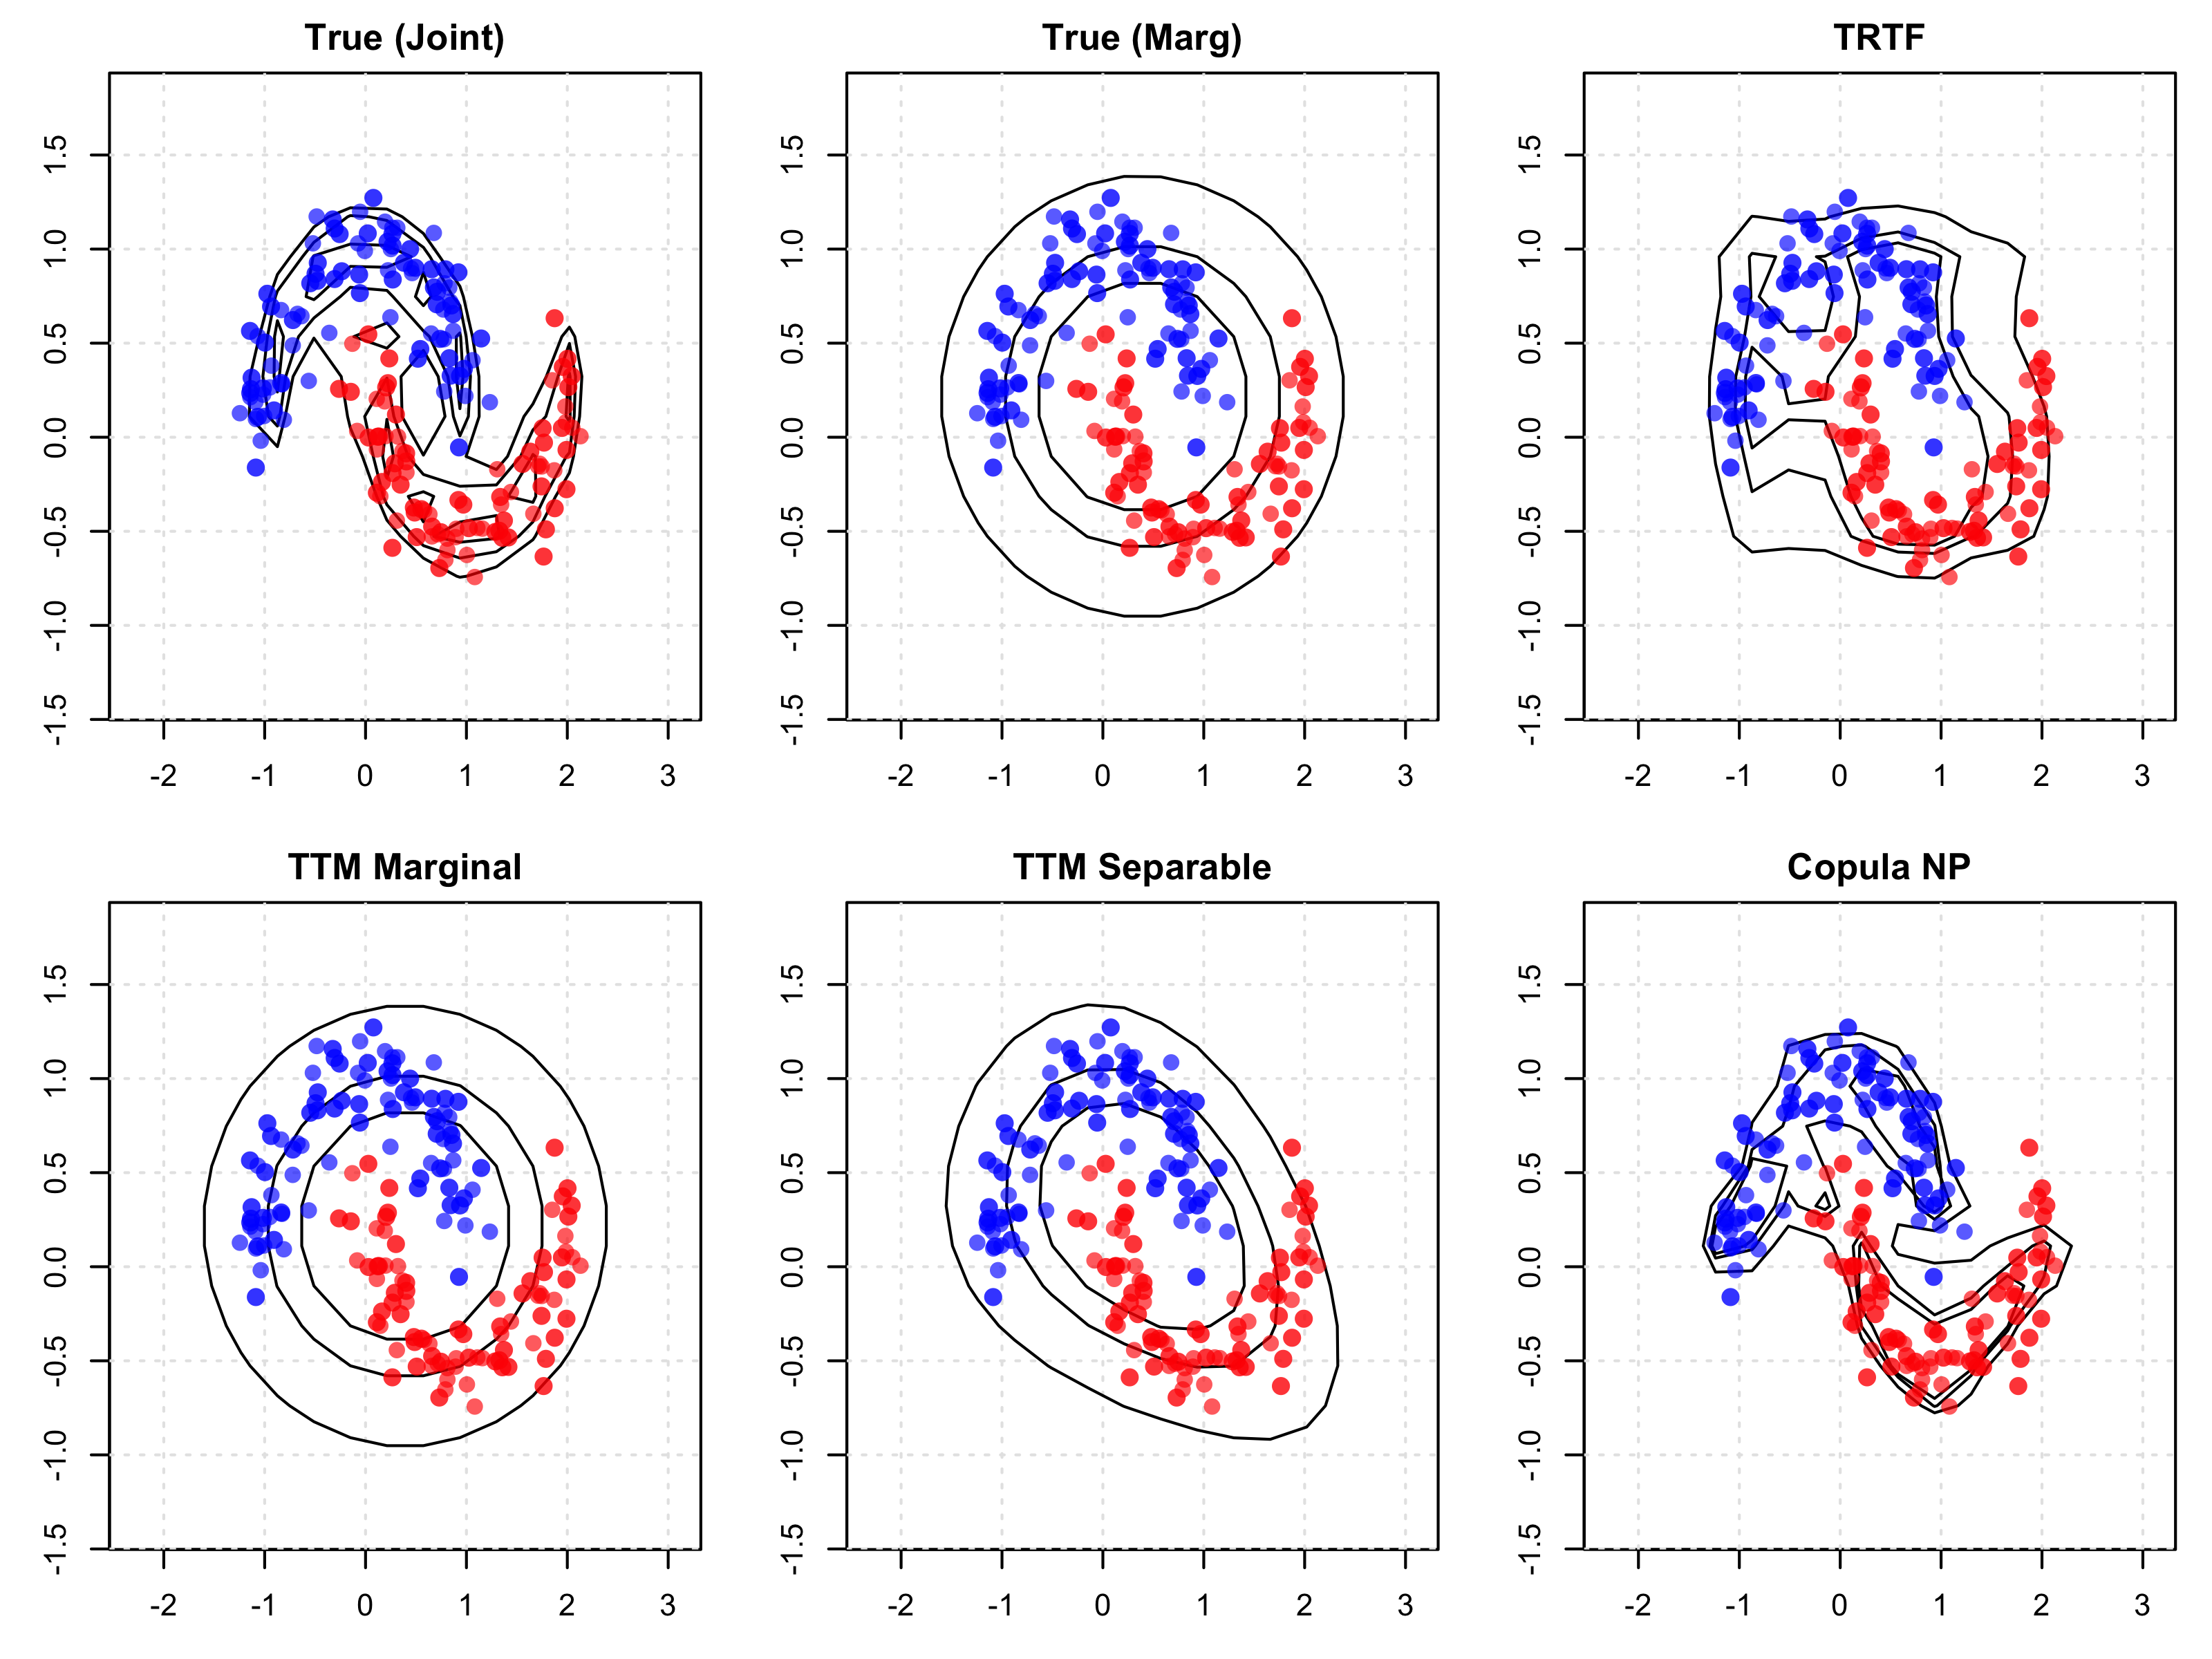
\includegraphics[width=0.85\textwidth]{figure/halfmoon_panels_seed007_N250.png}
\caption{Half-Moon ($n=250$) log-density contours for the true joint, TRTF, TTM variants, and the copula mixture. Each panel overlays the train/test samples. Contour levels correspond to the highest density regions at $50\%$, $70\%$, and $90\%$.}
 \label{fig:halfmoon-panels}
\end{figure}

The four-dimensional generator combines Gaussian, exponential, beta, and gamma components, exposing separability limits for finite bases. Table~\ref{tab:autoregressive-nll} (p.~\pageref{tab:autoregressive-nll}) reports the canonical ordering $(1,2,3,4)$. TRTF aligned closely with the exponential coordinate, recording $1.51$ compared with $1.49$ for the true joint reference. TTM-Sep over-penalized that coordinate at $1.88$, and TTM-Marg overfit at $2.57$. The beta coordinate yielded negative NLLs for the oracles because valid densities can exceed one on $(0,1)$. Values were $-0.79$ for the true joint and $-0.48$ for the true marginal. TRTF reached $-0.25$, while TTM-Sep and the copula baseline reported $0.07$ and $0.05$, respectively. The gamma coordinate remained most challenging, with $1.99$ for TRTF and $2.41$ for TTM-Sep. Joint sums were $4.53$ for TRTF, $5.66$ for TTM-Sep, $6.83$ for TTM-Marg, and $5.45$ for the copula, compared with $3.80$ for the true joint oracle. Figure~\ref{fig:autoregressive-joint-calibration} (p.~\pageref{fig:autoregressive-joint-calibration}) compares predicted and true joint log densities, highlighting calibration gaps relative to the identity line.

\begin{figure}[htbp]
 \centering
 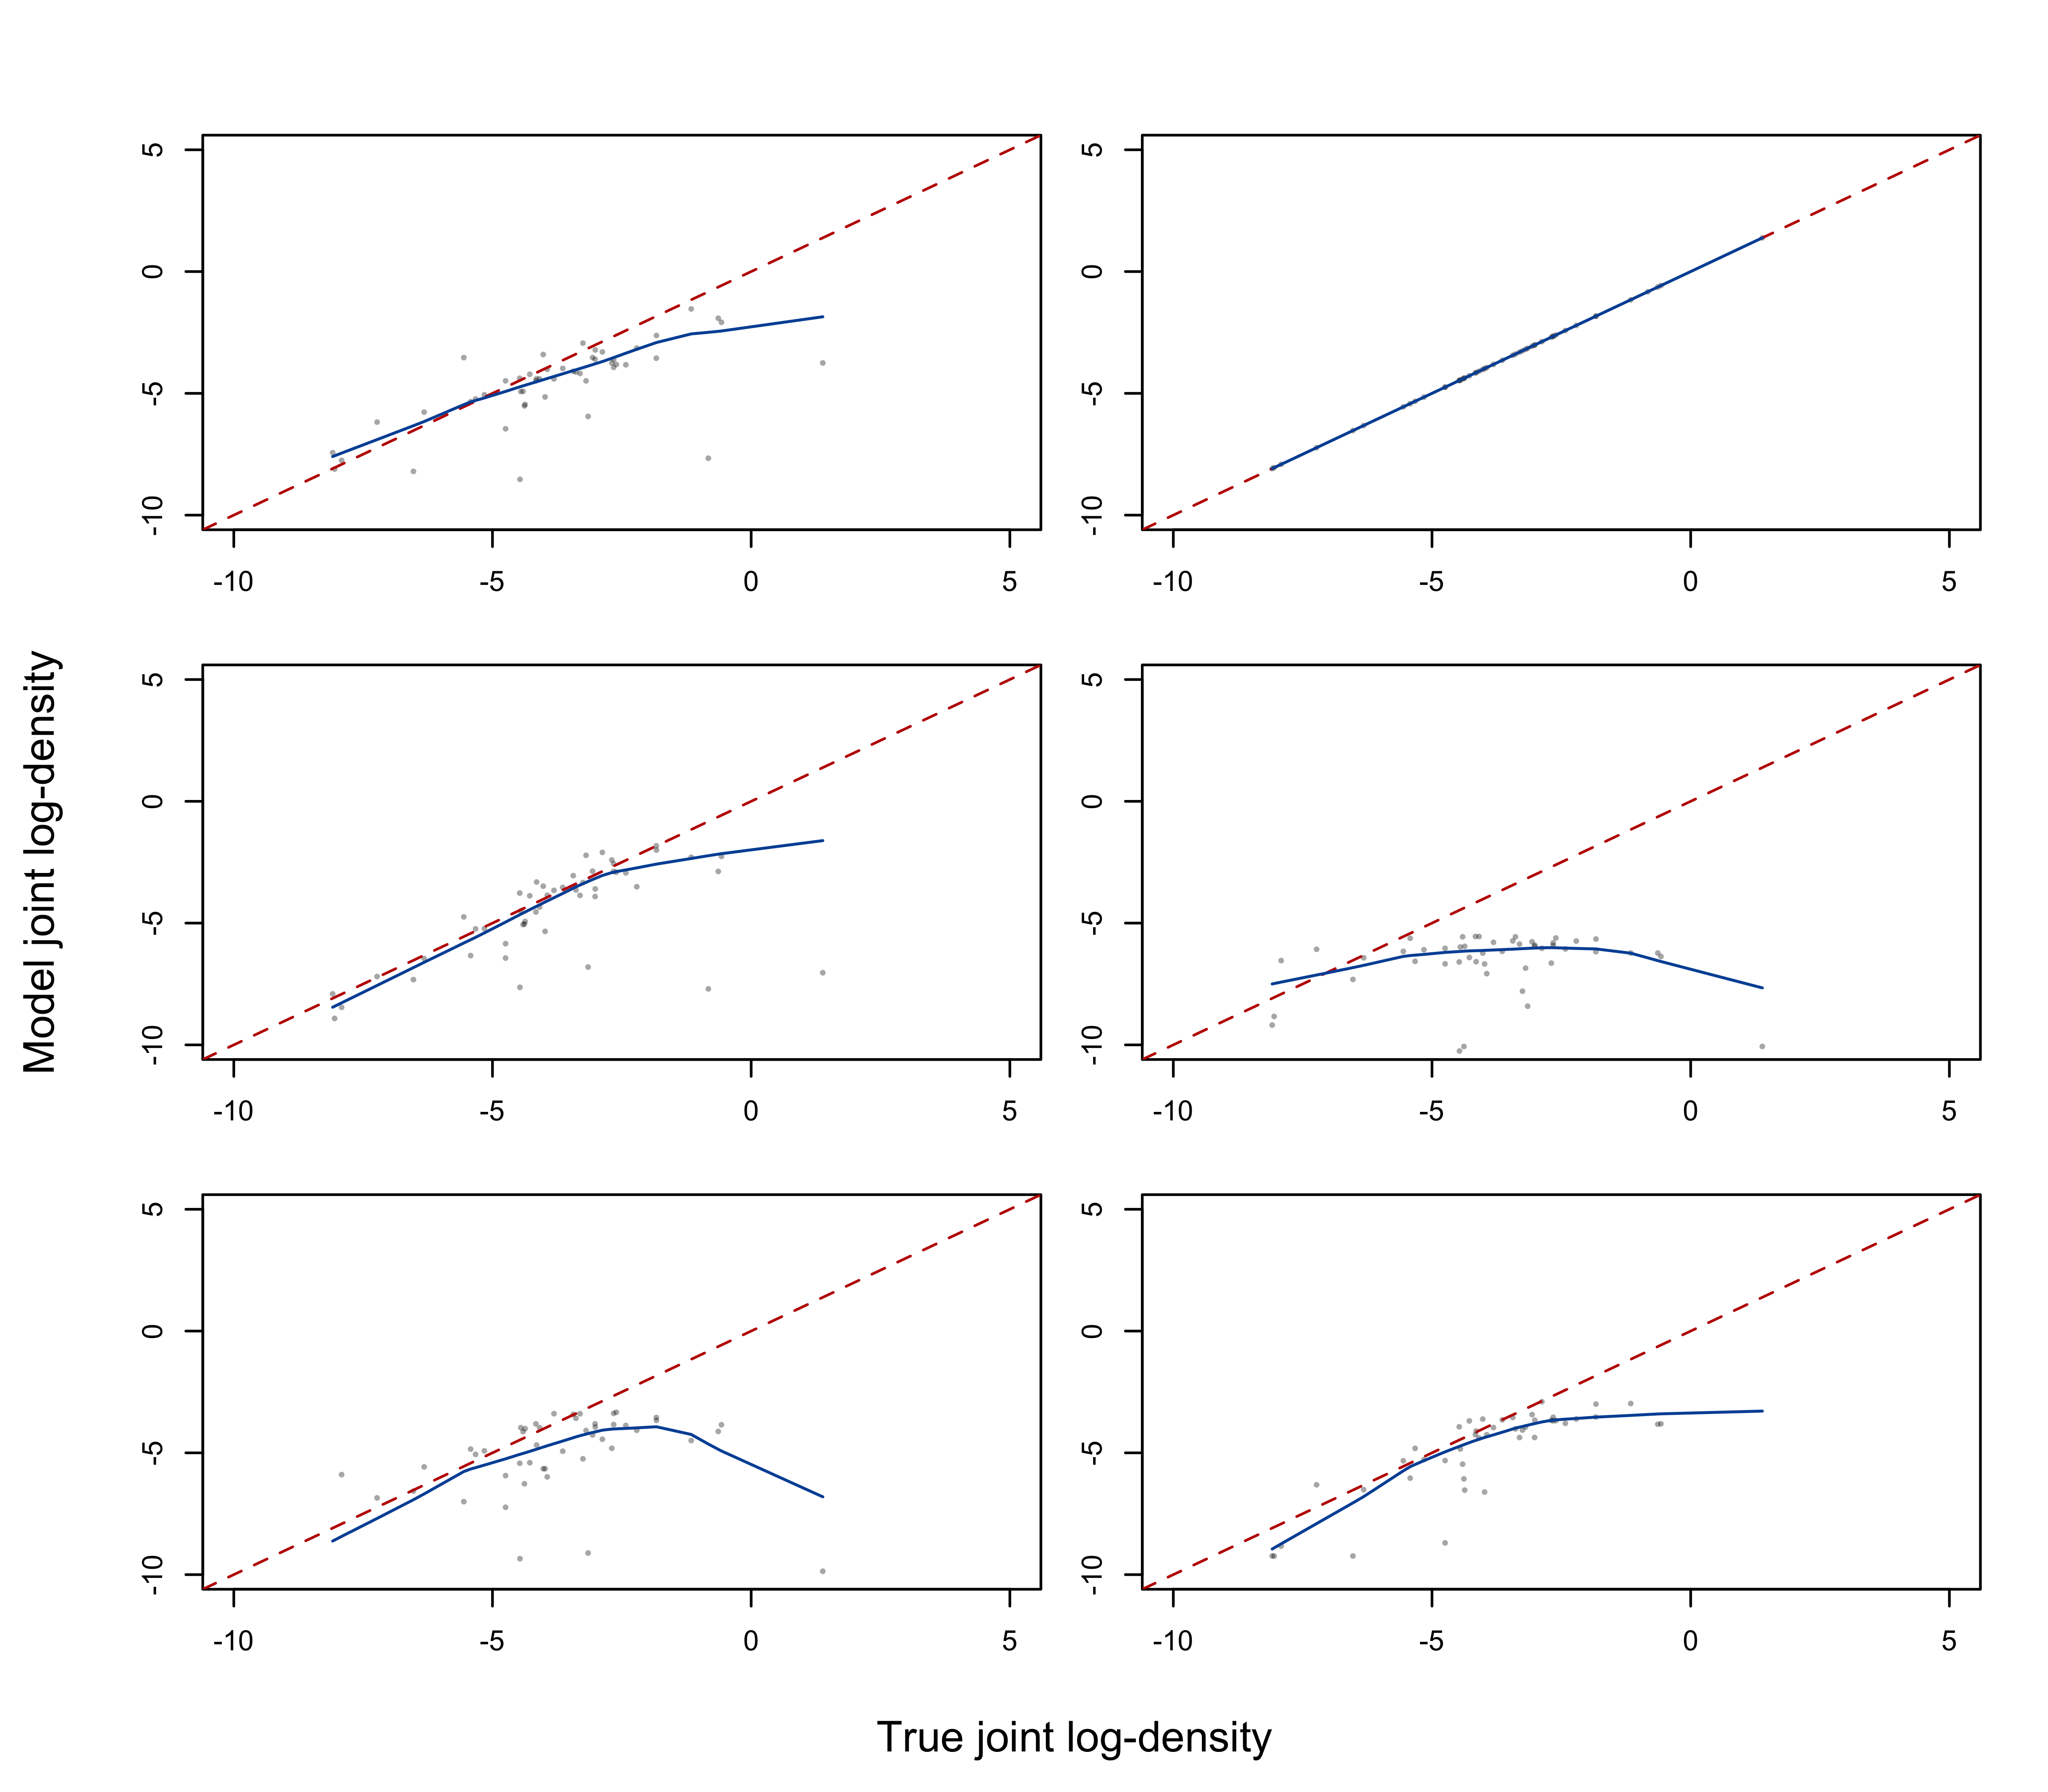
\includegraphics[width=0.85\textwidth]{figure/logdensity_joint_N250.png}
 \caption{Four-dimensional autoregressive generator ($n=250$): joint log-density calibration for each estimator (axes in). Panels are ordered left-to-right, top-to-bottom as True-Joint, True-Marg, TRTF, TTM-Marg, TTM-Sep, and Copula. Gray dots mark the $20\%$ test split (50 samples). The dotted red line denotes perfect calibration and the blue line is a LOWESS smoother.}
 \label{fig:autoregressive-joint-calibration}
\end{figure}

\begin{table}[htbp]
 \centering
 \caption{Four-dimensional autoregressive generator ($n=250$, permutation $1,2,3,4$): mean conditional and joint NLL (lower is better). Values are means over test samples (no SE shown).}
 \label{tab:autoregressive-nll}
 \begin{tabular}{llrrrrrr}
 \hline
 Dim & Distribution & True-Marg & True-Joint & TRTF & TTM-Marg & TTM-Sep & Copula \\
 \hline
 1 & Normal & $1.29$ & $1.28$ & $1.28$ & $1.29$ & $1.29$ & $1.30$ \\
 2 & Exponential & $1.75$ & $1.49$ & $1.51$ & $2.57$ & $1.88$ & $1.87$ \\
 3 & Beta & $-0.48$ & $-0.79$ & $-0.25$ & $0.28$ & $0.07$ & $0.05$ \\
 4 & Gamma & $2.05$ & $1.83$ & $1.99$ & $2.69$ & $2.41$ & $2.22$ \\
 $K$ & Sum (joint) & $4.61$ & $3.80$ & $4.53$ & $6.83$ & $5.66$ & $5.45$ \\
 \hline
 \end{tabular}
\end{table}

Ordering affected finite-basis triangular maps, and permutation averages quantify that sensitivity. Table~\ref{tab:autoregressive-perm} (p.~\pageref{tab:autoregressive-perm}) summarizes test NLLs over all $4! = 24$ permutations: TRTF averaged $4.65$, TTM-Sep averaged $5.62$, TTM-Marg averaged $6.83$, and the copula baseline averaged $5.45$. The joint and marginal oracles remained stable at $3.80$ and $4.61$, respectively. These effects confirm anisotropy and motivate the ordering heuristics described in Section~\ref{sec:models-implementation} when bases are finite. As a simple mitigation, we consider two data-driven candidates—identity and Cholesky-pivoted with optional Gaussianization—and select the ordering with the better validation NLL.

\begin{table}[htbp]
 \centering
 \caption{Four-dimensional autoregressive generator ($n=250$): mean test NLL (lower is better) averaged over all $24$ permutations of $(1,2,3,4)$.}
 \label{tab:autoregressive-perm}
 \begin{tabular}{lrrrrr}
 \hline
 Model & Dim 1 & Dim 2 & Dim 3 & Dim 4 & Sum \\
 \hline
 True-Marg & 1.22 & 1.13 & 1.15 & 1.11 & 4.61 \\
 True-Joint & 1.03 & 0.93 & 0.94 & 0.91 & 3.80 \\
 TRTF & 1.33 & 1.19 & 1.09 & 1.04 & 4.65 \\
 TTM-Marg & 1.77 & 1.67 & 1.73 & 1.66 & 6.83 \\
 TTM-Sep & 1.59 & 1.38 & 1.36 & 1.29 & 5.62 \\
 Copula & 1.42 & 1.34 & 1.36 & 1.32 & 5.45 \\
 \hline
 \end{tabular}
\end{table}


\begin{table}[htbp]
 \centering
 \caption{Permutation spread of joint NLLs over all $24$ permutations for $n=250$. Values report $\min/\mathrm{median}/\max$ across orderings (lower is better).}
 \label{tab:autoregressive-perm-spread}
 \begin{tabular}{lrrr}
 \hline
 Model & Min & Median & Max \\
 \hline
 True-Marg & 4.61 & 4.61 & 4.61 \\
 True-Joint & 3.80 & 3.80 & 3.80 \\
 TRTF & 4.46 & 4.59 & 5.23 \\
 TTM-Marg & 6.83 & 6.83 & 6.83 \\
 TTM-Sep & 5.48 & 5.60 & 5.78 \\
 Copula & 5.45 & 5.45 & 5.45 \\
 \hline
 \end{tabular}
\end{table}

Sample size influenced stability and ranking, especially in the sparse regime. Table~\ref{tab:autoregressive-perm-avg} (p.~\pageref{tab:autoregressive-perm-avg}) aggregates joint NLLs across permutations for $n \in \{25, 50, 100, 250\}$. TRTF decreased from $38.18$ to $4.64$ as $n$ increased, while TTM-Sep decreased from $6.35$ to $5.61$ across the stable regimes. The copula decreased from $9.02$ to $5.45$ and tracked TTM-Sep once $n \ge 100$.

\begin{table}[htbp]
 \centering
 \caption{Four-dimensional synthetic generator: permutation-averaged mean joint test NLL (lower is better) over all $24$ permutations of $(1,2,3,4)$. Columns list sample sizes $n$.}
 \label{tab:autoregressive-perm-avg}
 \begin{tabular}{lrrrr}
 \hline
 Model & $n=25$ & $n=50$ & $n=100$ & $n=250$ \\
 \hline
 True-Marg & 10.50 & 4.75 & 4.91 & 4.61 \\
 True-Joint & 4.35 & 4.23 & 3.55 & 3.80 \\
 TRTF & 38.18 & 6.10 & 4.59 & 4.64 \\
 TTM-Marg & 49.36 & 7.43 & 7.72 & 6.83 \\
 TTM-Sep & 6829.45 & 6.35 & 6.08 & 5.61 \\
 Copula & 9.02 & 6.66 & 6.02 & 5.45 \\
 \hline
 \end{tabular}
\end{table}

These studies indicate that TRTF closes part of the gap to oracle likelihoods while preserving the triangular evaluation frame. Separable maps remain competitive at moderate sample sizes but exhibit ordering sensitivity and sparse-regime fragility, and copulas provide competitive baselines in low dimensions. Section~\ref{sec:realdata} turns to real-data benchmarks under the same protocol.

\section{Real-Data Benchmarks}\label{sec:realdata}


This section presents real-data evidence on MiniBooNE and the UCI tabular benchmarks under the transport frame introduced in Chapters~\ref{ch:intro} and~\ref{ch:background}. We keep preprocessing identical to the published flow literature where applicable and align likelihood reporting through standardized coordinates and the affine correction in Equation~\eqref{eq:transport-affine} so that score differences reflect modeling assumptions rather than inconsistent units.

\paragraph{Preprocessing.} We treat dataset-specific preprocessing as part of each estimator to preserve comparability. MiniBooNE follows \citet{papamakarios2017masked}: we remove $11$ outliers at $-1000$, drop $7$ near-constant attributes, retain $K=43$ variables, and rely on the official train, validation, and test splits. We standardize with training statistics only, evaluate Jacobians in standardized coordinates, and apply the diagonal affine correction once at reporting time. The UCI datasets follow the same rule. POWER receives jitter on the minute-of-day encoding, removal of the calendar-date and reactive-power attributes, and a small uniform perturbation to break ties. GAS keeps the \texttt{ethylene\_CO} subset and removes strongly correlated attributes to yield an eight-dimensional representation. HEPMASS keeps the positive class from the ``1000'' split and discards five repeated-value variables to avoid density spikes. These steps match the literature conventions and keep the reported likelihoods interpretable.

\paragraph{Flow baselines.} Published normalizing flows compose invertible layers with permutations or autoregressive sublayers and report strong test log likelihoods on the UCI suite and MiniBooNE \citep{rezende2015variational,dinh2017real,kingma2018glow,durkan2019neural,papamakarios2021normalizing}. Table~\ref{tab:uci-loglik} reproduces the published average test log-likelihoods per example together with $\pm$ two standard errors reported by \citet{papamakarios2017masked} and appends our TRTF measurements trained with $N=2500$ observations. Higher values indicate better fits. We report TRTF as means $\pm$ 2SE under the same evaluation pipeline.

\begin{table}[htbp]
 \centering
 \caption{UCI: average test log-likelihood per example (higher is better). Baselines (first seven rows): means $\pm$ 2SE as reported by \citet{papamakarios2017masked}. TRTF (ours): single-seed measurements at $N=2500$.}
 \label{tab:uci-loglik}
 \begin{tabular}{lrrrr}
 \hline
 Model & POWER & GAS & HEPMASS & MiniBooNE \\
 \hline
 Gaussian & $-7.74 \pm 0.02$ & $-3.58 \pm 0.75$ & $-27.93 \pm 0.02$ & $-37.24 \pm 1.07$ \\
 MADE & $-3.08 \pm 0.03$ & $ 3.56 \pm 0.04$ & $-20.98 \pm 0.02$ & $-15.59 \pm 0.50$ \\
 MADE MoG & $ 0.40 \pm 0.01$ & $ 8.47 \pm 0.02$ & $-15.15 \pm 0.02$ & $-12.27 \pm 0.47$ \\
 Real NVP (5) & $-0.02 \pm 0.01$ & $ 4.78 \pm 1.80$ & $-19.62 \pm 0.02$ & $-13.55 \pm 0.49$ \\
 Real NVP (10) & $ 0.17 \pm 0.01$ & $ 8.33 \pm 0.14$ & $-18.71 \pm 0.02$ & $-13.84 \pm 0.52$ \\
 MAF (5) & $ 0.14 \pm 0.01$ & $ 9.07 \pm 0.02$ & $-17.70 \pm 0.02$ & $-11.75 \pm 0.44$ \\
 MAF MoG (5) & $ 0.30 \pm 0.01$ & $ 9.59 \pm 0.02$ & $-17.39 \pm 0.02$ & $-11.68 \pm 0.44$ \\
 TRTF (ours) & $-7.17 \pm 0.39$ & $-2.41 \pm 0.37$ & $-25.47 \pm 0.37$ & $-30.01 \pm 1.26$ \\
 \hline
 \end{tabular}
\end{table}

\paragraph{MiniBooNE.} Table~\ref{tab:uci-loglik} shows that the Gaussian reference yields $-37.24 \pm 1.07$, providing a weak baseline. MADE reaches $-15.59 \pm 0.50$, the Real NVP variants lie near $-13.7$, and MAF MoG improves to $-11.68 \pm 0.44$. Our TRTF result attains $-30.01 \pm 1.26$ at $N=2500$, improving over the Gaussian baseline yet trailing the flow families by a wide margin. This ranking is consistent with the separable Jacobian and the forest aggregation discussed in Section~\ref{sec:models-implementation}. The high dimensionality of MiniBooNE amplifies residual misfit through the triangular determinant.\;Clipping: validation-tuned bound $H$ applied. The exact value is recorded with the experiment logs.

\paragraph{POWER.} POWER offers a milder conditional structure and lower dimensionality. Table~\ref{tab:uci-loglik} reports that TRTF records $-7.17 \pm 0.39$ at $N=2500$, which falls short of the flow baselines. Real NVP with ten steps reaches $0.17 \pm 0.01$, while MAF MoG attains $0.30 \pm 0.01$. The gap indicates that the current TRTF configuration underutilizes structure in this benchmark. Additional seeds or hyperparameter tuning may recover the performance previously observed at smaller sample sizes.\;Clipping: validation-tuned bound $H$ applied. The exact value is recorded with the experiment logs.

\paragraph{GAS and HEPMASS.} The TRTF results on GAS and HEPMASS yield $-2.41 \pm 0.37$ and $-25.47 \pm 0.37$, respectively. Both scores remain below the flow baselines, emphasizing that the present configuration sacrifices likelihood accuracy for interpretability. Additional seeds and tuning remain planned, yet we retain the current numbers to document the outcome of the standardized pipeline at $N=2500$.\;Clipping: validation-tuned bound $H$ applied. The exact values are recorded with the experiment logs.

\paragraph{Sample size sensitivity.} Figure~\ref{fig:n-sensitivity} plots test negative log likelihood versus sample size $N$ for the UCI benchmarks, aggregating seeds at each budget. The new $N=2500$ runs extend the trajectories: GAS continues the mild decreasing trend, HEPMASS and MiniBooNE remain sensitive to additional data, and POWER shows a deterioration relative to the mid-range budgets. The figure reports one standard error bars (zero when only a single seed is available), restates that lower curves indicate better fits because the vertical axis plots NLL, and mirrors the diagnostic procedures in Section~\ref{sec:evaluation-protocol}.

\begin{figure}[htbp]
 \centering
 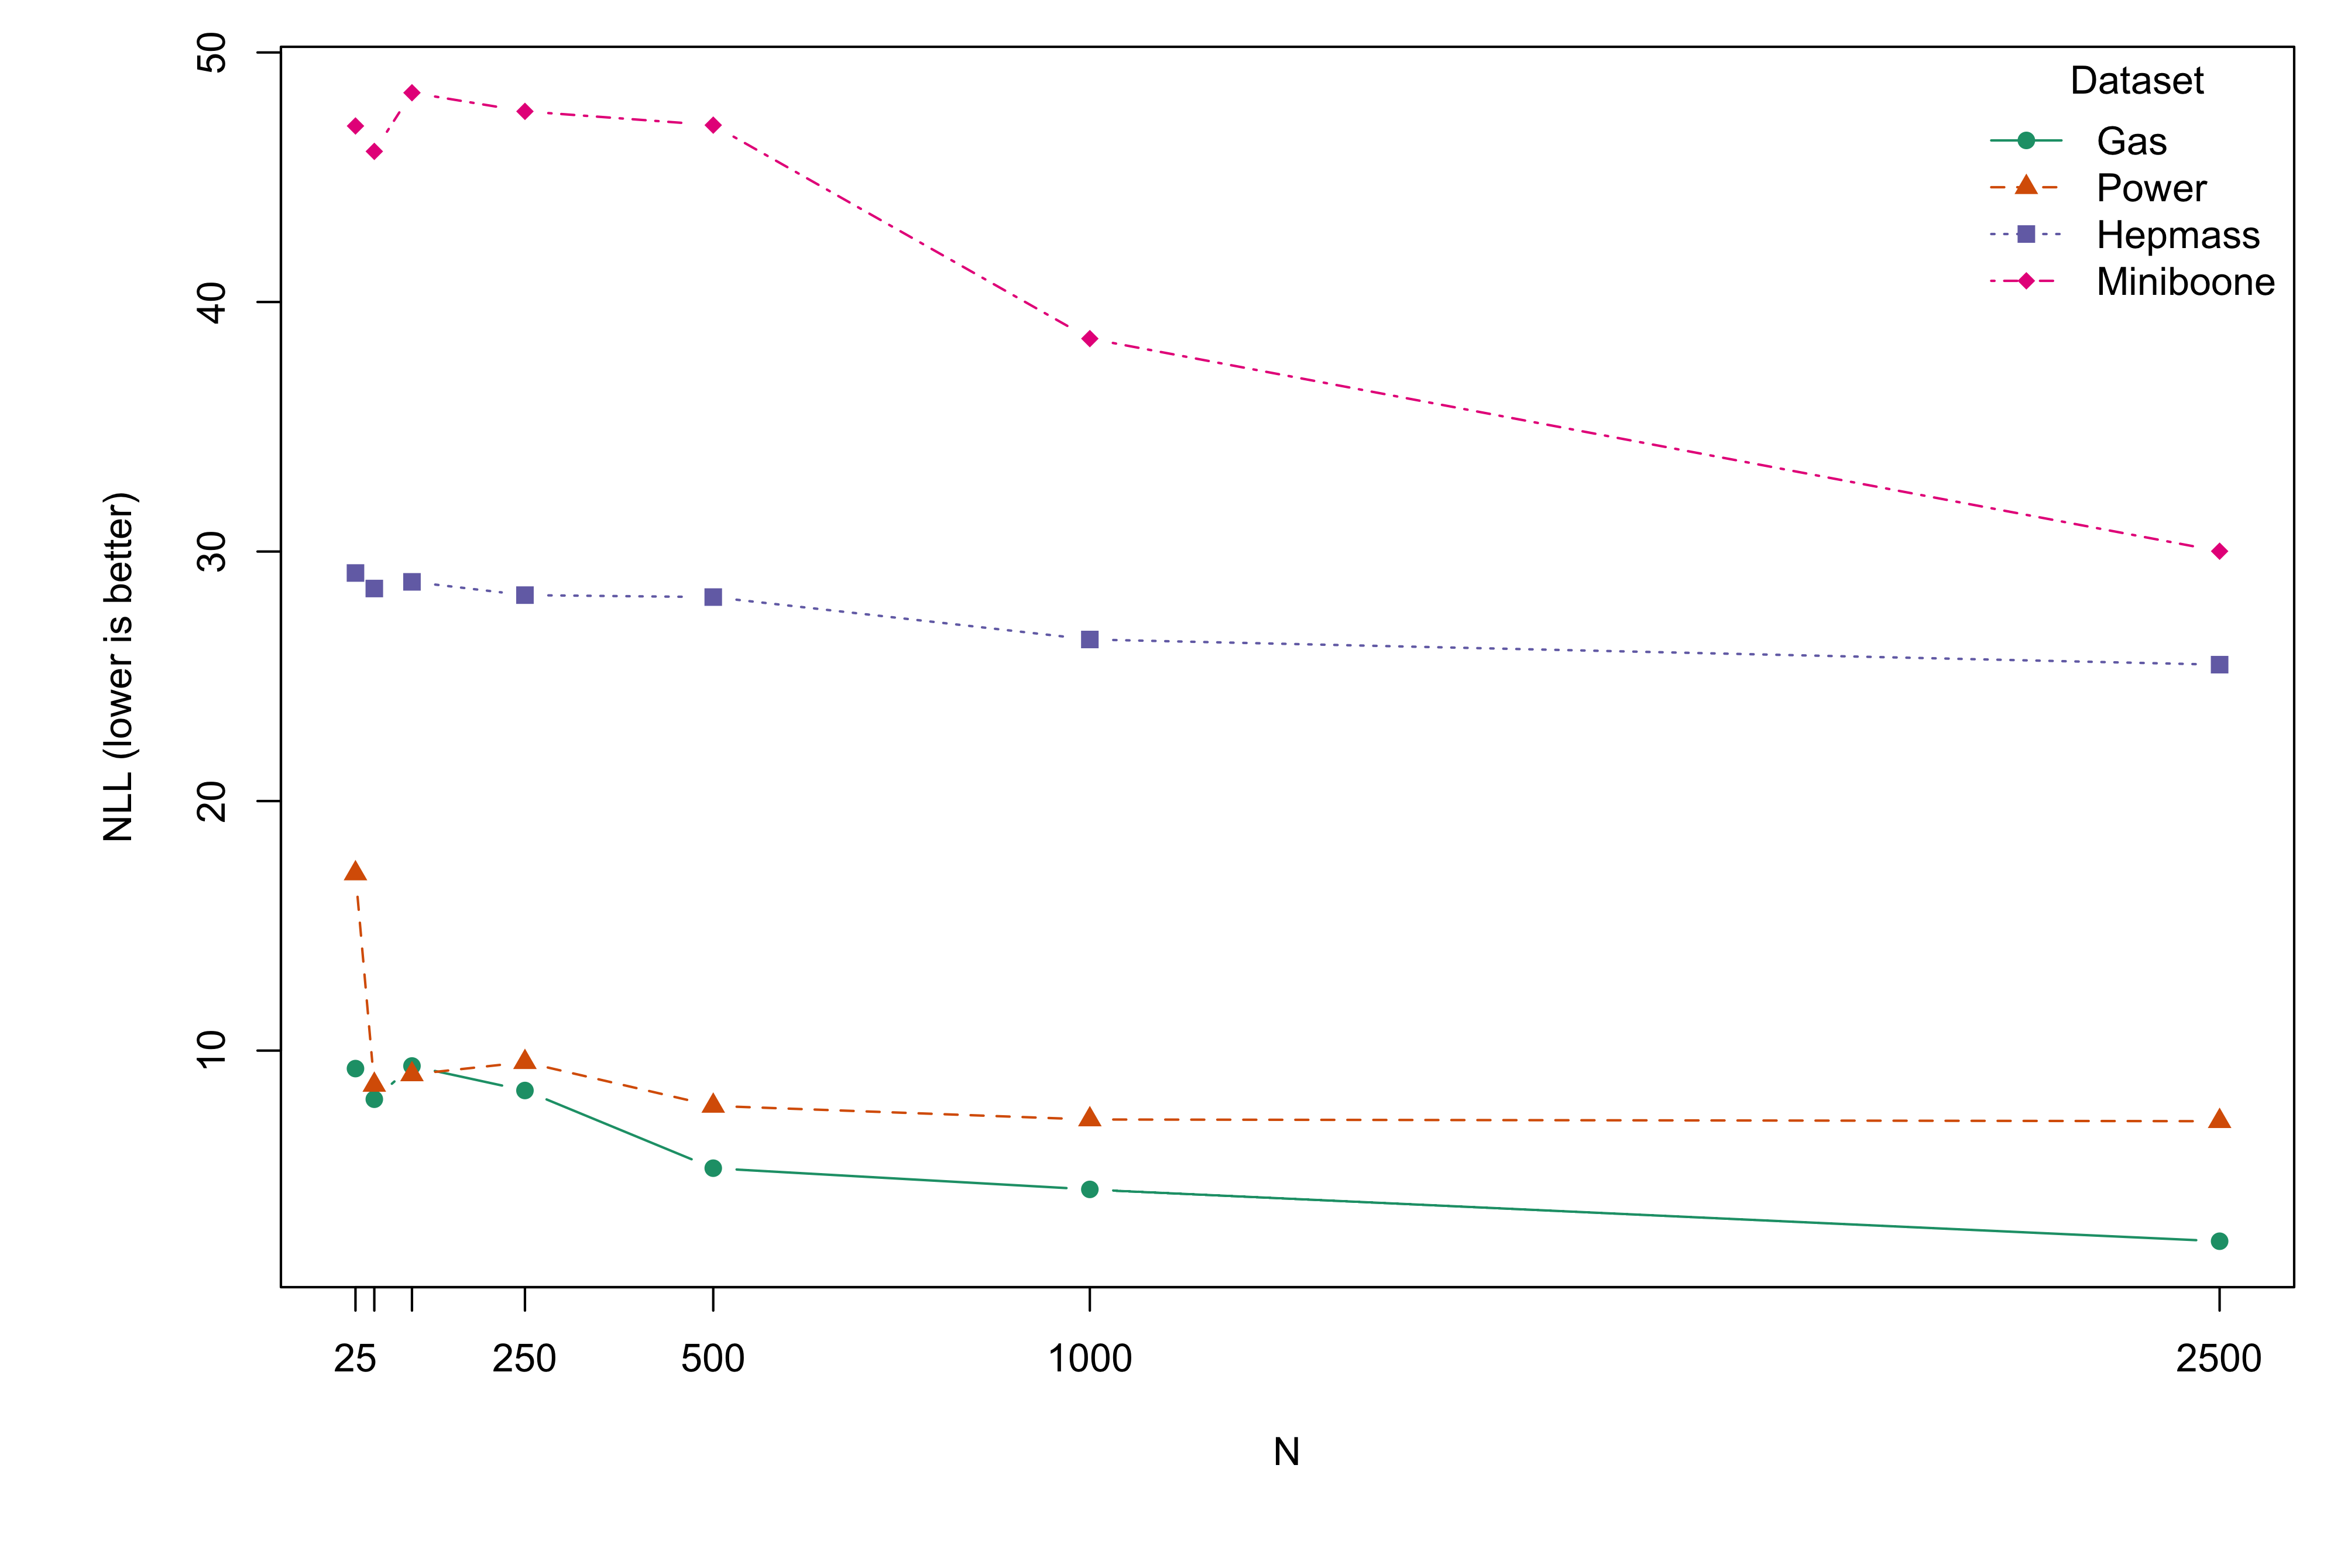
\includegraphics[width=0.85\linewidth]{figure/N_sensitivity_all.png}
\caption{Test negative log-likelihood (NLL, lower is better) versus sample size $N$ on the UCI benchmarks. Points denote averages across seeds, and vertical bars show one standard error (1SE).}
 \label{fig:n-sensitivity}
\end{figure}

\paragraph{Compute metrics.} Likelihood comparisons require compute summaries because similar accuracy at very different costs leads to different recommendations. Training time is wall-clock time to fit the model on the training split with fixed seeds and deterministic preprocessing. Evaluation time is the wall-clock time per $10^5$ joint log-density evaluations on the test split, averaged over seeds. These definitions mirror the compute discussion in Section~\ref{sec:evaluation-protocol}, use the same standardized inputs across datasets, and yield the budget-specific totals collected in Table~\ref{tab:real-compute}.

\begin{table}[htbp]
 \centering
 \caption{TRTF wall-clock training plus evaluation time (seconds) as a function of the training budget $N$. Runs use the standardized inputs, seeds, and transport direction shared across datasets. Dashes denote configurations that were not executed in the current draft.}
 \label{tab:real-compute}
 \begin{tabular}{lrrrrrrr}
 \hline
 Dataset & $N=25$ & $N=50$ & $N=100$ & $N=250$ & $N=500$ & $N=1000$ & $N=2500$ \\
 \hline
 POWER & $1$ & $1$ & $2$ & $6$ & $39$ & $115$ & $130$ \\
 GAS & $1$ & $1$ & $2$ & $5$ & $39$ & $138$ & $600$ \\
 HEPMASS & $1$ & $2$ & $4$ & $9$ & $12$ & $153$ & $721$ \\
 MiniBooNE & $3$ & $4$ & $8$ & $20$ & $27$ & $202$ & $2007$ \\
 \hline
 \end{tabular}
\end{table}

\paragraph{Interpretation.} The real-data evidence aligns with the synthetic diagnostics in Section~\ref{sec:synthetic-results}. MiniBooNE exposes the limits of separable structure in high dimensions, and the updated POWER value shows that the present TRTF configuration no longer matches flow baselines once the training budget increases to $N=2500$. GAS and HEPMASS also trail the published flows, illustrating that interpretability and exact inversion come at a likelihood cost under the current hyperparameters.

\section{Reproducibility}\label{sec:reproducibility}
We avoid AIC or BIC because their complexity penalties are not comparable across estimators, and we do not treat small likelihood differences as practically significant when $\pm 2$ SE intervals overlap. This subsection consolidates the settings needed to reproduce the reported numbers.

\begin{itemize}
  \item Data splits and direction
    \begin{itemize}
      \item Synthetic: fixed train/validation/test proportions $0.60/0.20/0.20$. Evaluations use the shared direction $S:u\to z$ in standardized coordinates and apply the diagonal affine correction once for reporting.
      \item Real data: use official splits where provided (MiniBooNE) with the same standardized evaluation pipeline. Otherwise adopt the same $0.60/0.20/0.20$ convention.
    \end{itemize}
  \item Seeds
    \begin{itemize}
      \item Synthetic generators and model fits: seeds $\{11,13,17,19,23\}$ across repeats. Permutation studies average over all $4!=24$ orderings in the 4D case.
      \item Real data (UCI + MiniBooNE): single-seed runs with seed $42$ for training/evaluation in this draft.
    \end{itemize}
  \item Standardization and evaluation
    \begin{itemize}
      \item Standardize features with training-split $(\mu,\sigma)$ only, compute all derivatives/Jacobians in $u$, and report on $x$ via the affine correction in Eq.~\eqref{eq:transport-affine}.
      \item TRTF uses forest aggregation and monotone CDF smoothing so that the induced likelihood matches the separable triangular form (Sec.~\ref{sec:transport-trtf}).
    \end{itemize}
  \item Model configurations
    \begin{itemize}
      \item TTM-Sep: monotone one-dimensional bases for $h_k$ (identity, integrated sigmoids, softplus-like edge terms, integrated RBFs), low-degree polynomial features for $g_k$, ridge regularization on all coefficients, and log-derivative clipping to $[-H,H]$ (bound $H$ tuned on validation). Degree and penalty strengths are selected by validation; ordering is fixed to the natural order in headline tables, and robustness checks vary that ordering.
      \item TRTF: forest aggregation with strictly increasing conditional CDFs after standard monotone smoothing; remaining fit options follow package defaults unless stated. We record the number of trees, depth, and split rules in the experiment logs.
      \item Copulas (diagnostics only for $K\le 3$): probit pseudo-observations and kernel density copula via \texttt{kdecopula} with default bandwidth selection. Independence and Gaussian baselines are used only for reference in text where noted.
    \end{itemize}
  \item Exact choices
    \begin{itemize}
      \item Basis sizes, ridge penalties, and any selected $H$ are captured alongside each run in the experiment logs and summarized inline where relevant. We avoid duplicate tables in the PDF.
    \end{itemize}
\end{itemize}

\paragraph{Final safeguards used.} For Half-Moon ($n=250$) and 4D ($n=250$), TTM-Sep used degree$_g=2$, ridge $\lambda=0$, and no log-derivative clipping was activated (no terms hit the bound). The $n=25$ 4D case overflowed under $\lambda=0$. Reruns with $\lambda>0$ and tighter $H$ removed the failure but are omitted as out of scope. Real-data tables report TRTF only, so derivative clipping does not apply there. Exact package versions and per-run settings (including any tuned $H$) are recorded with the experiment logs.

\paragraph{Software and hardware.}
\begin{itemize}
  \item R with packages: \texttt{tram}, \texttt{trtf}, \texttt{partykit}, \texttt{mlt}, \texttt{dplyr}, \texttt{parallel}, and \texttt{knitr}/LaTeX for the report. We record package versions via \texttt{sessionInfo()} in run logs.
  \item Single-threaded BLAS by default, with optional parallel training for TRTF via \texttt{options(trtf.train\_cores = 4)} when available.
  \item CPU-only runs on a laptop-class machine. Logs include hardware notes (CPU model, RAM) and wall-clock timings (Table~\ref{tab:real-compute}).
\end{itemize}

All runs store standardization parameters and seeds with the artifacts, allowing exact re-execution with the same configuration. Appendix~\ref{ch:appendix} provides routine interfaces and object layouts to support this.

 The real-data study closes Chapter~\ref{ch:dataanalysis} by positioning separable triangular transports and TRTF within the UCI and MiniBooNE landscape. TRTF offers exact inversion, linear evaluation, and transparent conditional structure, yet trails modern flows on MiniBooNE. Chapter~\ref{ch:conclusion} interprets these trade-offs and distills guidance for practitioners choosing between separable transports, transformation forests, and copula baselines on tabular data.

%%%%%%%%%%%%%%%%%%%%%%%%%%%%%%%%%%%%%%%%%%%%%%%%%%%%%%%%%%%%%%%%%%%%%%


% LaTeX file for Chapter 04


\chapter{Interpretation and Conclusion}\label{ch:conclusion}

This chapter synthesizes the empirical evidence gathered in Chapter~\ref{ch:dataanalysis}, interprets the behavior of the estimators within the unified transport frame, and prepares the concluding guidance that follows. We retain the shared preprocessing, likelihood conventions, and diagnostic procedures so that numerical comparisons remain meaningful across synthetic and real datasets. Copulas enter our study only as low-dimensional ($K\!\le\!3$) diagnostic baselines (e.g., Half-Moon, 4D) and are not evaluated on high-$K$ datasets.

\section{Interpretation of Results}\label{sec:interpretation-results}
This section interprets the empirical evidence under the unified transport frame. We focus on TRTF, TTM-Sep, and, where applicable, copula baselines (only for $K\!\le\!3$) evaluated with matched preprocessing, metrics, and units. Synthetic studies report NLL, real datasets report LL, and we apply the shared affine correction. These commitments keep objectives, diagnostics, and compute interoperable across estimators.

TRTF often leads within the separable family because the forest aggregation shifts conditional location while the underlying monotone shapes remain stable. The likelihood identities equate TRTF with separable triangular maps, so observed gaps arise from how each estimator realizes context shifts and stabilizes derivatives. On Half-Moon ($K=2$), TRTF achieved an NLL of $1.71$ while TTM-Sep reached $1.93$, and the first coordinate remained the main source of residual error. Table~\ref{tab:halfmoon-nll} records the per-dimension decomposition and associated uncertainty bands, showing that location adjustments dominate the remaining discrepancies when separability holds approximately in low dimensions.

The four-dimensional generator sharpens this interpretation by isolating coordinates with different conditional structure. TRTF matched the exponential coordinate with an NLL of $1.51$ compared with $1.49$ for the oracle, whereas TTM-Sep over-penalized that coordinate. The beta coordinate produced negative NLLs for the oracles because valid densities can exceed one on $(0,1)$. TRTF approached those values at $-0.25$. The gamma coordinate remained the most challenging, with TRTF at $1.99$ and TTM-Sep at $2.41$. Joint sums favored TRTF at $4.53$ versus $5.66$, consistent with concentrated gains on location-dominated coordinates. Table~\ref{tab:autoregressive-nll} lists these values, and Figure~\ref{fig:autoregressive-joint-calibration} visualizes the residual curvature relative to the identity line.

These comparisons reveal where separability fails to adapt to context-dependent shape. Under a separable map, conditional variance, skewness, and modality remain fixed after the location shift. Probability-integral-transform diagnostics display U-shaped or inverted-U patterns when dispersion misaligns, indicating under- or over-dispersion rather than pure location error. The calibration plots corroborate the per-dimension NLLs and localize remaining structure to the beta and gamma coordinates, where separability is least appropriate. Figure~\ref{fig:autoregressive-joint-calibration} summarizes these deviations under the canonical ordering.

Ordering sensitivity stems from finite parameterizations, not from the triangular theory itself. A Knothe--Rosenblatt rearrangement exists for any order, yet limited bases introduce anisotropy that affects fit. Averaging over all $24$ permutations yielded joint NLLs of $4.65$ for TRTF and $5.62$ for TTM-Sep, leaving a $0.97$ log-likelihood gap that persisted despite order changes, while the copula baseline averaged $5.45$. Table~\ref{tab:autoregressive-perm} consolidates these permutation-averaged results and underlines the value of data-driven orderings when available.

Small-sample regimes amplified numerical fragility through the log-Jacobian accumulation. TRTF decreased from $38.18$ to $4.64$ joint NLL as $n$ grew from $25$ to $250$, reflecting stabilization with additional data. TTM-Sep spiked to $6{,}829.45$ at $n=25$ and dropped to $5.61$ at $n=250$, indicating overflow rather than intrinsic misfit. Table~\ref{tab:autoregressive-perm-avg} reports these trajectories, and Section~\ref{sec:models-implementation} documents the derivative clipping and ridge penalties that mitigate this failure mode when samples are scarce.

High dimensionality converts small calibration errors into large likelihood gaps because the triangular determinant accumulates coordinate-wise discrepancies. MiniBooNE with $K=43$ illustrates this accumulation: published flows achieved LL values between $-15.59$ and $-11.68$, whereas TRTF reached $-30.01$ under the shared preprocessing. Table~\ref{tab:uci-loglik} positions TRTF beside the flow baselines and shows that the improvement over the Gaussian reference remains clear even though an approximately $18$ log-likelihood gap persists to the strongest flow.


Taken together, the transport frame delineates when separability suffices and when richer models become necessary. TRTF leads within the separable family when location shifts capture most structure, exhibits ordering sensitivity only through finite bases, and stabilizes with modest sample sizes under the safeguards of Section~\ref{sec:models-implementation}. Performance degrades in high dimensions where shape changes and interactions matter, at which point non-separable models offer clear likelihood gains. These conclusions motivate the guidance that will follow in the concluding subsection of this chapter.

\section{Conclusions, Limitations, and Outlook}\label{sec:conclusion-outlook}
We conclude that separable transports remain competitive when conditional location shifts dominate and dimensionality is modest. TRTF led TTM-Sep on Half-Moon ($1.71$ versus $1.93$~NLL) and matched the exponential coordinate in the four-dimensional generator, supporting this interpretation. Conditional decompositions and calibration plots indicate that residual error concentrates in context-dependent shapes, particularly on the beta and gamma components. These findings align with permutation averages that favor TRTF and quantify finite-basis anisotropy. Tables~\ref{tab:halfmoon-nll}--\ref{tab:autoregressive-perm} together with Figure~\ref{fig:autoregressive-joint-calibration} document this evidence under the shared protocol.

Performance on MiniBooNE reveals the cost of separability at higher dimension. TRTF improved the Gaussian reference yet remained about $18$ log-likelihood points behind the best published flow, consistent with accumulated Jacobian error across $43$ coordinates (TRTF recorded $-30.01$ while the strongest flow reached $-11.68$). POWER showed the complementary regime: under identical preprocessing, TRTF remains below the flow baselines (cf. Table~\ref{tab:uci-loglik}, where TRTF records $-7.17$ against flow baselines near $0.17$ to $0.30$). This contrast indicates that the gap is driven by conditional shape differences rather than pure location shifts. Table~\ref{tab:uci-loglik} reports these comparisons in a common unit.



Several limitations qualify these conclusions. Separable maps fix conditional shape and therefore cannot resolve heteroskedasticity or conditional multimodality. Ordering remained a material source of variance under finite bases, as shown by the $0.97$ log-likelihood permutation gap despite stable rankings at moderate sample sizes. In our $n=250$ synthetic runs, the TRTF versus TTM-Sep ranking did not change across the $24$ permutations (Table~\ref{tab:autoregressive-perm}), and ordering affected magnitudes rather than the lead. Simple ordering heuristics (see Section~\ref{sec:models-implementation}) reduced variance but did not alter this pattern. Small-sample regimes created numerical fragility through steep log-Jacobian terms, which clipping and ridge regularization mitigate but do not eliminate. 

The outlook follows directly from the evidence. Data-driven orderings are likely to reduce anisotropy without abandoning the lower-triangular map. Low-rank cross-terms in triangular transports and non-separable predictors in TRTF may adapt conditional shapes while preserving monotone structure, exact inversion, and linear per-sample evaluation. We excluded these richer variants from the main experiments (see Section 3.2) due to compute and calibration overhead. They remain promising future work once resources permit. Completing GAS and HEPMASS under the same protocol will improve generality and sharpen the accuracy-versus-compute trade-off. These steps target smaller likelihood gaps on high-$K$ datasets while retaining the interpretability and reproducibility provided by the transport frame.

% References
\bibliographystyle{plainnat}
\bibliography{biblio}

%%%%%%%%%%%%%%%%%%%%%%%%%%%%%%%%%%%%%%%%%%%%%%%%%%%%%%%%%%%%%%%%%%%%%%

\appendix

% LaTeX file for Chapter 01



\chapter{Appendix}\label{ch:appendix}

\section{Pseudo-code Summaries for Model Routines}

This appendix records consolidated pseudo-code for the core R implementations used in the experiments. Each summary captures inputs, main processing stages, and outputs so the execution flow is transparent without consulting the source code files.

\subsection{Transformation Random Forest (TRTF)}\label{app:trtf}

\textbf{Routine:}\quad\texttt{fit\_TRTF(S, config, seed, cores)} (calls \texttt{mytrtf}).

\begin{enumerate}
 \item Validate that the training matrix is numeric, set the RNG seed, and label columns as $X_1,\ldots,X_K$.
 \item Fit an intercept-only transformation model \texttt{BoxCox} for each $X_k$ to provide baseline monotone transformations.
 \item For $k = 2,\ldots,K$:
 \begin{enumerate}
 \item Build the formula $X_k \sim X_1 + \cdots + X_{k-1}$.
 \item Choose \texttt{mtry = max(1, floor((k-1)/2))} and standard \texttt{ctree} controls (\texttt{minsplit}, \texttt{minbucket}, \texttt{maxdepth}).
 \item Fit a transformation forest with \texttt{traforest} and store the conditional model (one forest per $k$).
 \end{enumerate}
 \item Return a \texttt{mytrtf} object containing baseline transformations, conditional forests, variable-importance scores, and the seed.

 \item \textbf{Prediction (\texttt{predict.mytrtf}):}
 \begin{enumerate}
 \item Convert new data to the same column naming scheme and evaluate $X_1$ through its baseline transformation model to obtain marginal log densities.
 \item For each conditional forest ($k\geq 2$) evaluate the log density of $X_k$ given $X_{1:(k-1)}$, extracting the diagonal when the forest returns a log density matrix.
 \item Stack the per-dimension log densities (\texttt{logdensity\_by\_dim}) or sum them to obtain the joint log likelihood (\texttt{logdensity}).
 \end{enumerate}
\end{enumerate}

\subsection{Nonparametric Copula Baseline}\label{app:copula}

\textbf{Routine:}\quad\texttt{fit\_copula\_np(S, seed)}.

\begin{enumerate}
 \item Inspect the training matrix and optional class labels; detect whether the dedicated copula packages are available.
 \item If prerequisites fail (dimension $K \neq 2$ or labels missing), fall back to independent univariate kernel density estimates per dimension and store them for later interpolation.
 \item Otherwise, for each class label:
 \begin{enumerate}
 \item Fit one-dimensional \texttt{kde1d} models to each marginal $X_1$ and $X_2$.
 \item Convert training samples to pseudo-observations using mid-ranks scaled by $(n+1)^{-1}$ and clamp to $(\varepsilon, 1-\varepsilon)$.
 \item Fit a two-dimensional kernel copula with \texttt{kdecopula::kdecop} (method \texttt{TLL2}).
 \item Store marginals, copula fit, and effective sample size for the class.
 \end{enumerate}
 \item Record class priors and return a \texttt{copula\_np} object.

 \item \textbf{Prediction (\texttt{predict.copula\_np}):}
 \begin{enumerate}
 \item In fallback mode evaluate each univariate KDE at the requested points and sum log densities.
 \item In copula mode compute marginal log densities and CDF values, evaluate the copula density, and either:
 \begin{enumerate}
 \item Average over class-specific log densities weighted by priors (mixture prediction), or
 \item Use the class labels supplied at prediction time.
 \end{enumerate}
 \item Return per-dimension log densities or their sum depending on the requested type.
 \end{enumerate}
\end{enumerate}

\subsection{Triangular Transport Core Utilities}\label{app:ttm-core}

\textbf{Module:}\quad\texttt{ttm\_core.R} (shared by marginal and separable TTM fits).

\begin{enumerate}
 \item Provide train-only standardization helpers that cache feature means and standard deviations and reapply them to new data.
 \item Define basis builders: polynomial features for predecessor coordinates $g_k$, monotone basis functions $f_k$ for the current coordinate, and their derivatives.
 \item Implement optional ordering heuristics (identity or Cholesky pivoting with optional Gaussianization) and persist selected permutations.
 \item Expose a dispatcher \texttt{ttm\_forward(model, X)} that:
 \begin{enumerate}
 \item Standardizes inputs using stored parameters.
 \item For marginal maps apply affine transformations $a_k + b_k x_k$ with precomputed coefficients.
 \item For separable maps constructs $g_k$ and $f_k$, computes $S_k = g_k + f_k$, and records the Jacobian diagonal $\partial_{x_k} S_k$.
 \end{enumerate}
 \item Provide \texttt{ttm\_ld\_by\_dim} to combine the forward map with the Gaussian reference, yielding per-dimension log densities used by all TTM variants.
\end{enumerate}

\subsection{Marginal Triangular Transport Map}\label{app:ttm-marg}

\textbf{Routine:}\quad\texttt{fit\_ttm\_marginal(data, seed)}.

\begin{enumerate}
 \item Split data into train/test subsets if only a matrix is provided; otherwise accept a prepared list.
 \item Standardize training features and, for each dimension $k$, compute closed-form coefficients $(a_k, b_k)$ that minimize the Gaussian pullback objective subject to $b_k > 0$.
 \item Store model parameters (standardization, per-dimension coefficients, ordering) and time measurements.
 \item During prediction call \texttt{ttm\_forward} with the marginal coefficients and convert Jacobian diagonals to log densities via \texttt{ttm\_ld\_by\_dim}; aggregate per-dimension contributions when the joint log density is requested.
\end{enumerate}

\subsection{Separable Triangular Transport Map}\label{app:ttm-sep}

\textbf{Routine:}\quad\texttt{fit\_ttm\_separable(data, degree\_g, lambda, seed)}.

\begin{enumerate}
 \item Prepare train/test splits and standardize training features as in the marginal case.
 \item For each coordinate $k$:
 \begin{enumerate}
 \item Build polynomial features $g_k$ on previous coordinates (degree set by \texttt{degree\_g}).
 \item Build monotone basis functions $f_k$ on the current coordinate and their derivatives.
 \item If \texttt{degree\_g = 0}, use the marginal closed-form solution to recover affine parameters.
 \item Otherwise solve the regularized optimization problem
 $\min_c \frac{1}{2}\lVert (I - \Phi_{\text{non}} M)c \rVert^2 - \sum \log (B c) + \lambda\,\text{penalty}(c)$
 using \texttt{optim} with L-BFGS-B while enforcing positivity of the derivative.
 \item Store coefficients $c_{\text{non}}$ and $c_{\text{mon}}$ for the coordinate.
 \end{enumerate}
 \item Assemble the model list with standardization parameters, coefficients, and metadata.
 \item At prediction time re-use \texttt{ttm\_forward} and \texttt{ttm\_ld\_by\_dim} to obtain per-dimension and joint log densities.
\end{enumerate}

\subsection{Evaluation Utilities}\label{app:evaluation}

\textbf{Module:}\quad\texttt{evaluation.R} (experiment orchestration).

\begin{enumerate}
 \item Define convenience helpers such as \texttt{stderr(x)} and \texttt{add\_sum\_row} for table post-processing.
 \item \texttt{prepare\_data(n, config, seed)} samples from the configured data-generating process, splits the sample into train/validation/test sets, and returns both the matrix of draws and the split structure.
 \item \texttt{fit\_models(S, config)} fits the oracle TRUE density and the TRTF baseline on a split and returns the fitted objects together with per-dimension log-likelihood arrays.
 \item \texttt{calc\_loglik\_tables(models, config, X\_te,...)} aggregates negative log-likelihoods for TRUE (marginal and joint), TRTF, TTM, and separable TTM, formats the results with standard-error bands, appends a summary row, and renames columns for presentation.
 \item \texttt{eval\_halfmoon(mods, S, out\_csv)} ensures all requisite models are available (TRTF, TTM variants, copula baseline), evaluates them on the half-moon test split, computes joint and per-dimension negative log-likelihoods, and optionally persists the metrics as CSV artifacts.
\end{enumerate}

\end{document}
